\documentclass{article}
\usepackage{fullpage}

%load needed packages
\usepackage{graphicx}
\usepackage{array}
\usepackage{booktabs}
\usepackage[utf8]{inputenc}
\usepackage[T1]{fontenc}
\usepackage{url}
\usepackage[spanish]{babel} % Paquete para el idioma español
\usepackage{float}  % Necesario para [H]
\usepackage{listings}
\usepackage{xcolor}

\definecolor{codegreen}{HTML}{5AB2FF}
\definecolor{morado}{HTML}{AD88C6}
\definecolor{BG}{HTML}{EEEEEE}
\definecolor{azul}{HTML}{4D869C}
\definecolor{sqlblue}{HTML}{FF8C00} % Color para las palabras clave SQL

% Estilo para DDL
\lstdefinestyle{ddlstyle}{
	language=SQL,
	backgroundcolor=\color{BG},
	commentstyle=\color{codegreen},
	basicstyle=\ttfamily\small,
	keywordstyle=\color{azul},
	stringstyle=\color{morado},
	showstringspaces=false,
	breaklines=true,
	frame=shadowbox,
	numbers=left,
	numberstyle=\tiny\color{gray},
	captionpos=b,
}

% Estilo para SQL
\lstdefinestyle{sqlstyle}{
	language=SQL,
	backgroundcolor=\color{BG},
	commentstyle=\color{codegreen},
	basicstyle=\ttfamily\small,
	keywordstyle=\color{sqlblue}, % Color diferente para palabras clave SQL
	stringstyle=\color{morado},
	showstringspaces=false,
	breaklines=true,
	frame=shadowbox,
	numbers=left,
	numberstyle=\tiny\color{gray},
	captionpos=b,
}

\begin{document}
	
	
	
	% Portada
	\begin{titlepage}
		\centering
		\vspace*{3cm}
		
		% Título destacado
		{\Huge \textbf{Análisis de datos (MDX)}\\[0.5cm]}
		
		% Espacio y logotipo (si lo tienes, por ejemplo el logo de tu universidad)
		\vspace{2cm}
		
\includegraphics[width=0.3\textwidth]{images/uma_logo.jpg}\\[1cm]
		
		% Nombre del autor
		{\LARGE \textbf{Alejandro Silva Rodríguez}\\[0.5cm]}
		{\LARGE \textbf{Marta Cuevas Rodríguez}\\[0.5cm]}
		{\large \textit{Almacenes De Datos}\\
			Universidad de Málaga\\
		}
		
		\vfill
		
		% Fecha en la parte inferior de la página
		{\large Diciembre 2024}
	\end{titlepage}
	
	% indice
	\tableofcontents
	
	\newpage
\section{Introducción}
\label{sec:introduccion}

En el contexto hospitalario actual, el análisis avanzado de datos se ha convertido en una herramienta indispensable para optimizar la toma de decisiones y mejorar la gestión de recursos en áreas críticas como las Unidades de Cuidados Intensivos (UCI). El análisis detallado del gasto en medicamentos, que representa una proporción significativa de los costos operativos, requiere técnicas especializadas que permitan explorar grandes volúmenes de datos desde múltiples perspectivas.\\

Tras la construcción de un almacén de datos orientado al análisis del gasto en medicamentos, el siguiente paso lógico es implementar estructuras que soporten consultas analíticas avanzadas. Los cubos multidimensionales permiten una visión integral de los datos, facilitando la identificación de patrones, tendencias y áreas críticas de gasto. Además, el uso de consultas MDX (Multidimensional Expressions) habilita a los usuarios para realizar análisis dinámicos y obtener insights clave de manera rápida y eficiente. Este trabajo se centra en la creación y explotación de un cubo multidimensional diseñado específicamente para analizar el gasto en medicamentos en pacientes ingresados en UCI en hospitales de EE.UU. \cite{eicu_crd}

\section{Objetivos}
\label{sec:objetivos}

El objetivo principal de este trabajo es diseñar, implementar y explotar un cubo multidimensional para analizar el gasto en medicamentos en las UCI mediante el uso de consultas MDX. Este propósito se concreta en los siguientes objetivos específicos:

\begin{itemize}
	\item Diseñar y construir un cubo multidimensional que permita explorar de manera eficiente el gasto en medicamentos desde múltiples dimensiones, como tiempo, tipo de medicamento y características del paciente.
	\item Implementar consultas MDX que permitan realizar análisis detallados.

\end{itemize}










\section{Creación del Cubo Multidimensional}
En esta sección se explicará el proceso de creación del cubo multidimensional a partir del almacén de datos cargado, de manera detallada.

\subsection{Pasos Iniciales}
Para comenzar con el proyecto, abre Visual Studio y crea un nuevo proyecto de tipo \textbf{Proyecto Multidimensional de Analysis Services}, como se muestra en la figura \ref{fig:plantilla}.

\begin{figure}[H]
	\begin{center} 
		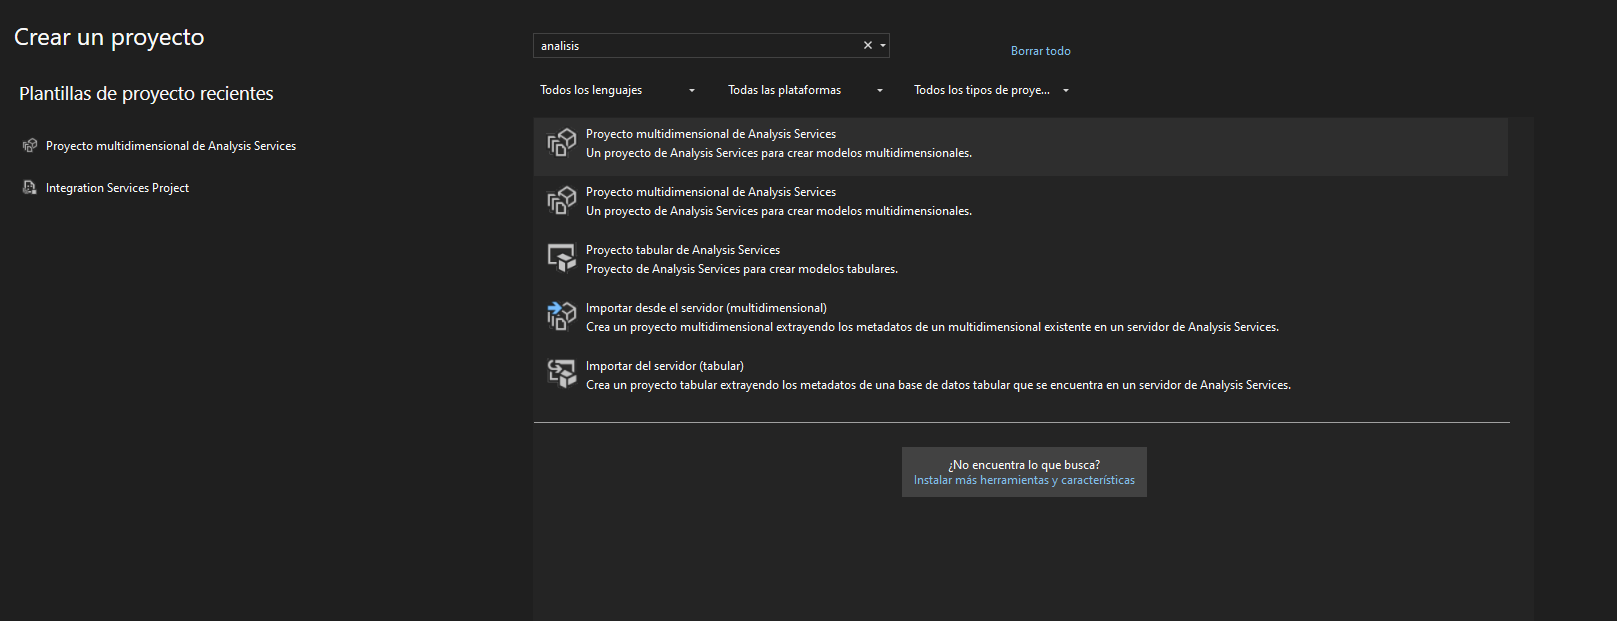
\includegraphics[width=\textwidth]{images/plantilla.png}
		\caption{Creación de un nuevo proyecto multidimensional en Visual Studio.}
		\label{fig:plantilla}
	\end{center}
\end{figure}

\subsection{Creación del Origen de Datos}
El siguiente paso consiste en crear un nuevo \textbf{Origen de Datos}. Para ello, selecciona la opción de crear una nueva conexión, como se muestra en la figura \ref{fig:conexion}. Posteriormente, configura la conexión con \textbf{Autenticación SQL Server}, utilizando una cuenta de servicio.

\begin{figure}[H]
	\begin{center} 
		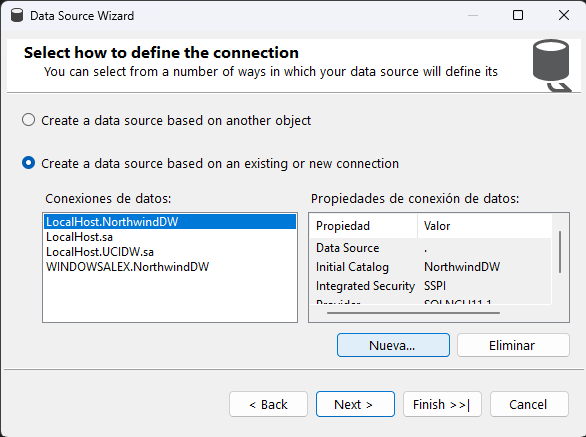
\includegraphics[width=.7\textwidth]{images/conexion.png}
		\caption{Nueva conexión en Visual Studio.}
		\label{fig:conexion}
	\end{center}
\end{figure}

\subsubsection{Configuración de la Conexión}
A continuación, selecciona \textbf{Autenticación SQL Server} y utiliza la cuenta de servicio para configurar la conexión a la base de datos.

\begin{figure}[H]
	\centering
	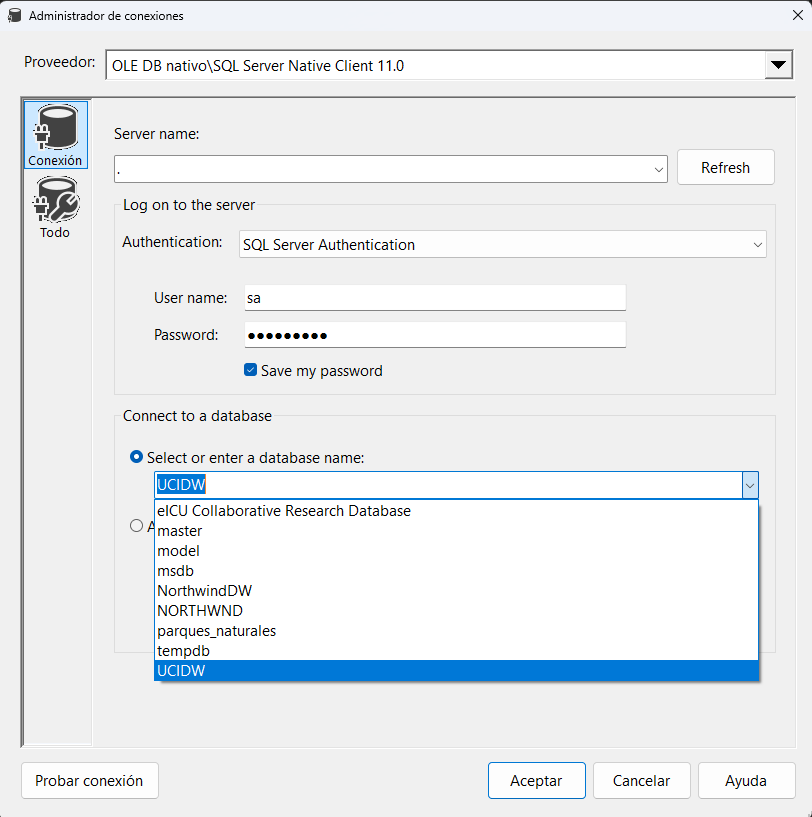
\includegraphics[width=0.7\linewidth]{images/conexion_bd.png}
	\caption{Configuración de la autenticación SQL Server.}
	\label{fig:conexion2}
\end{figure}

\subsection{Creación de la Vista de Origen de Datos}
Una vez configurada la conexión, creamos una nueva vista de origen de datos. Para ello, seleccionamos el origen de datos previamente configurado, tal como se muestra en la figura \ref{fig:origen}.

\begin{figure}[H]
	\begin{center} 
		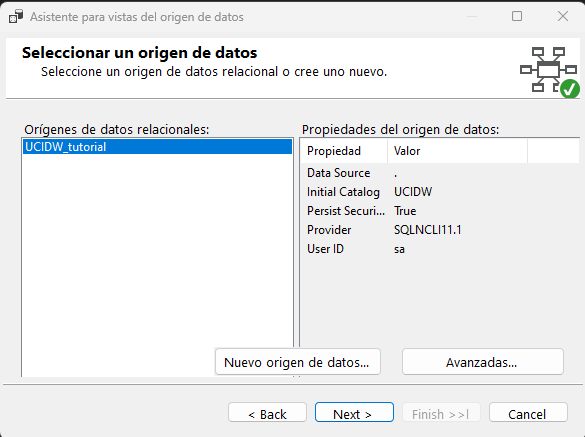
\includegraphics[width=.7\textwidth]{images/vista1.png} 
		\caption{Selección del origen de datos configurado previamente.}
		\label{fig:origen}
	\end{center}
\end{figure}

A continuación, seleccionamos las tablas necesarias del origen de datos.

\begin{figure}[H]
	\begin{center} 
		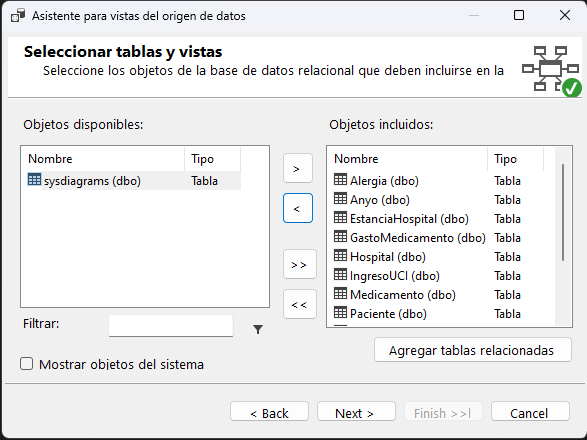
\includegraphics[width=.7\textwidth]{images/vista_tablas.png}
		\caption{Selección de tablas del origen de datos.}
		\label{fig:origen2}
	\end{center}
\end{figure}

Verifica la vista de la base de datos para asegurarte de que todas las tablas estén correctamente configuradas.

\begin{figure}[H]
	\begin{center} 
		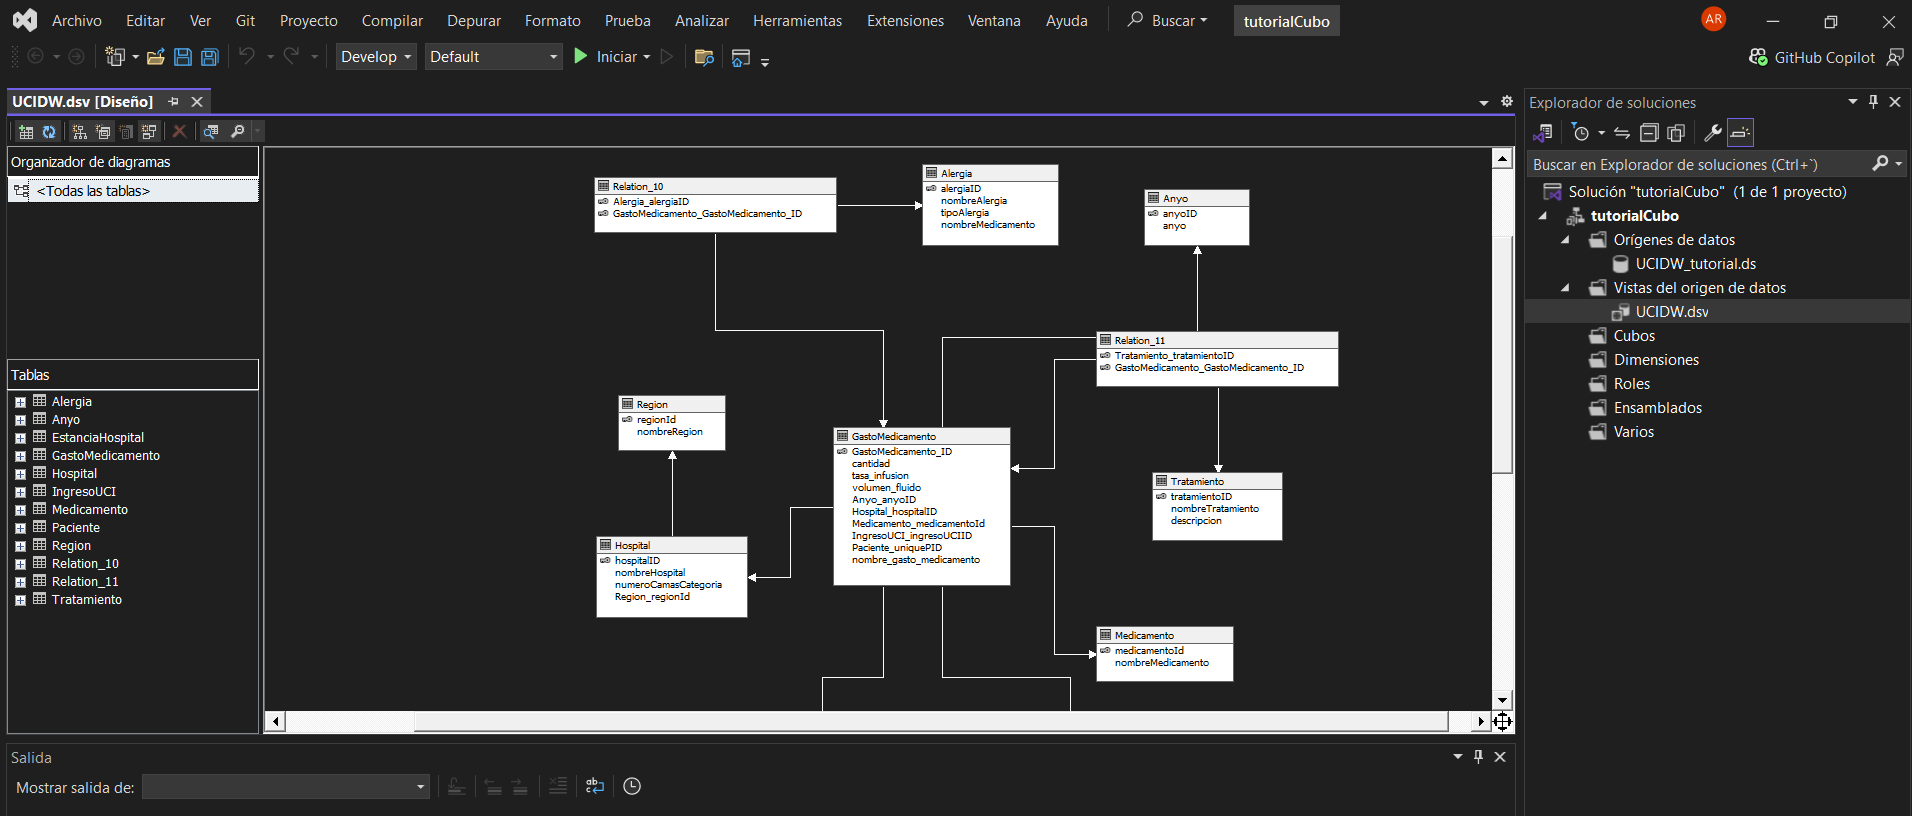
\includegraphics[width=.9\textwidth]{images/vista_imagen.png}
		\caption{Verificación de la vista de la base de datos.}
		\label{fig:origen3}
	\end{center}
\end{figure}

\subsection{Creación del Cubo}
Una vez configuradas las tablas, procede a crear el cubo multidimensional utilizando las tablas seleccionadas. En la figura \ref{fig:cubo1} se muestra el proceso de creación del cubo.

\begin{figure}[H]
	\begin{center} 
		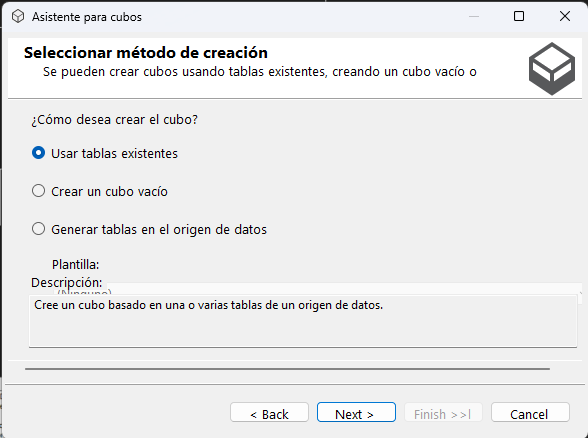
\includegraphics[width=.7\textwidth]{images/cubo1.png} 
		\caption{Creación del cubo multidimensional con las tablas seleccionadas.}
		\label{fig:cubo1}
	\end{center}
\end{figure}

En este paso, seleccionamos las tablas del grupo de medida, como el \textbf{Gasto de Medicamento}, y los grupos de medida intermedios para las relaciones de tipo NM, como se muestra en la figura \ref{fig:cubo_medidas}.

\begin{figure}[H]
	\begin{center} 
		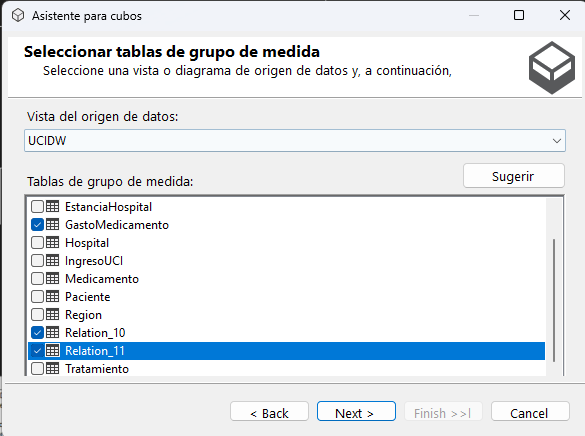
\includegraphics[width=.7\textwidth]{images/cubo_medidas.png} 
		\caption{Selección de tablas del grupo de medida y relaciones intermedias.}
		\label{fig:cubo_medidas}
	\end{center}
\end{figure}

Luego, seleccionamos las medidas y dimensiones del cubo, como se puede ver en la figura \ref{fig:dimensiones} y \ref{fig:medidas}.

\begin{figure}[H]
	\begin{center} 
		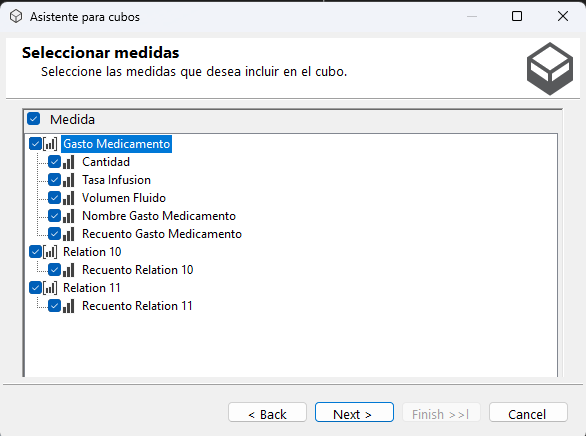
\includegraphics[width=.7\textwidth]{images/medidas2.png} 
		\caption{Configuración de medidas.}
		\label{fig:medidas}
	\end{center}
\end{figure}
\begin{figure}[H]
	\begin{center} 
		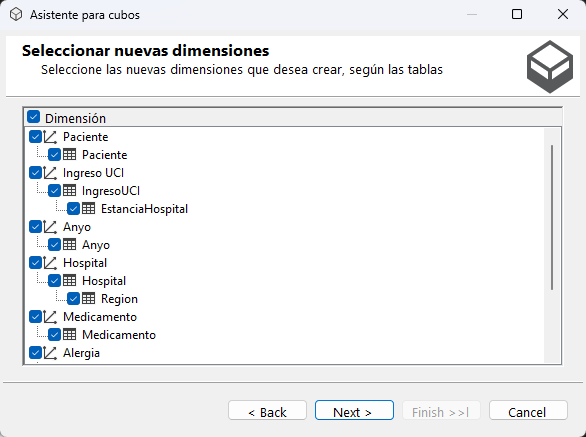
\includegraphics[width=.7\textwidth]{images/dimensiones.png} 
		\caption{Configuración dimensiones en el cubo.}
		\label{fig:dimensiones}
	\end{center}
\end{figure}

Finalmente, visualizamos el cubo creado en la figura \ref{fig:cubo_vista}.

\begin{figure}[H]
	\begin{center} 
		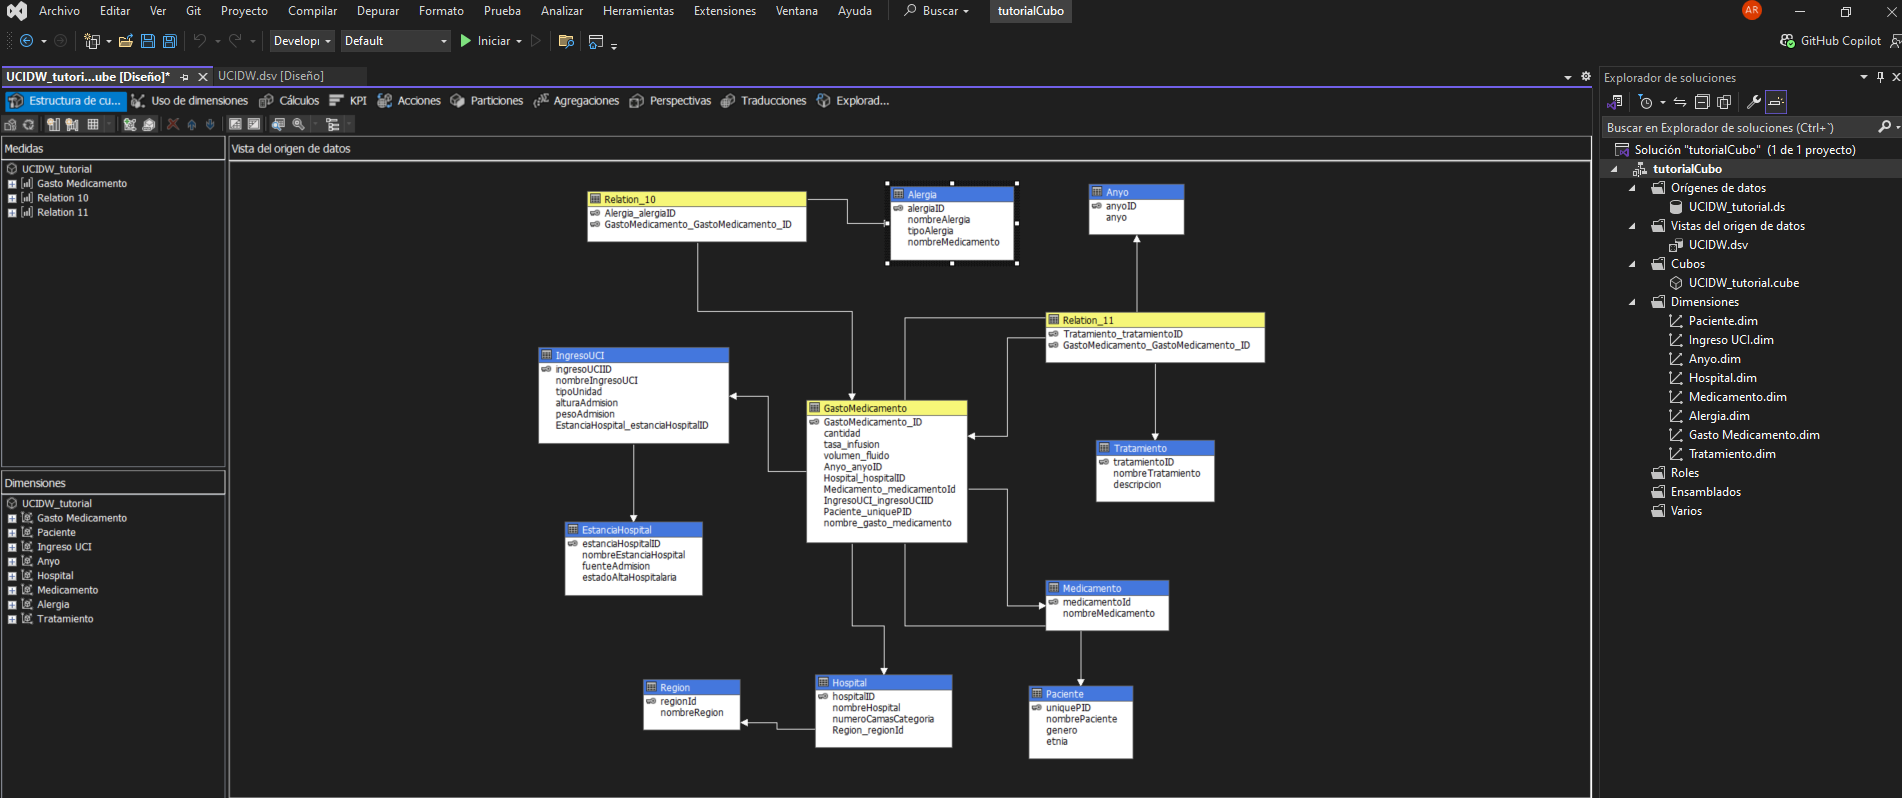
\includegraphics[width=.9\textwidth]{images/cubo_vista.png} 
		\caption{Visualización del cubo.}
		\label{fig:cubo_vista}
	\end{center}
\end{figure}
\subsection{Relaciones y Dimensiones}
Para configurar las relaciones, vamos a \textbf{Uso de Dimensiones}, donde definimos las relaciones entre el \textbf{Gasto} y el \textbf{Gasto}  de tipo Hecho, así como las relaciones entre las dimensiones NM y los grupos de medidas intermedio. La figura \ref{fig:uso_hecho} muestra este proceso.

\begin{figure}[H]
	\begin{center} 
		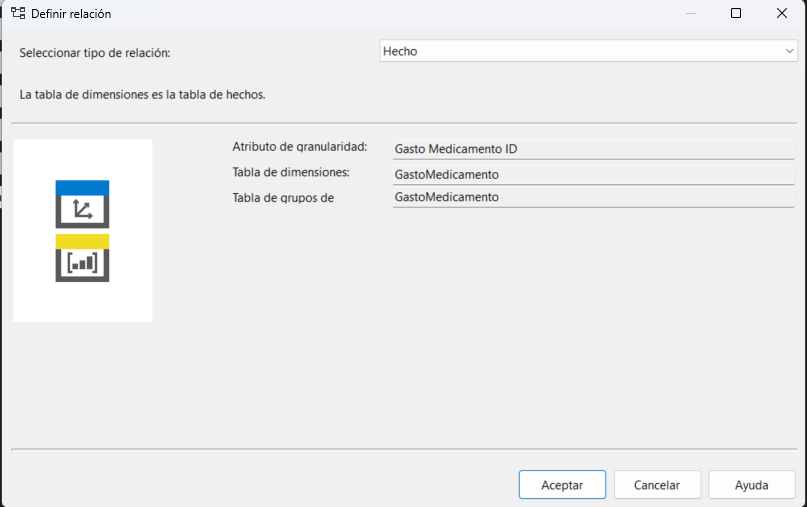
\includegraphics[width=.7\textwidth]{images/uso_hecho.png} 
		\caption{Relacion entre dimension Gasto y grupo de medidas Gasto de tipo Hecho}
		\label{fig:uso_hecho}
	\end{center}
\end{figure}

Además, configuramos relaciones de tipo \textbf{Varios a Varios} para dimensiones como \textbf{Alergia} y \textbf{Tratamiento}, con \textbf{Gasto de Medicamento}, como se muestra en las figuras \ref{fig:relation10} y \ref{fig:relation11}.

\begin{figure}[H]
	\begin{center} 
		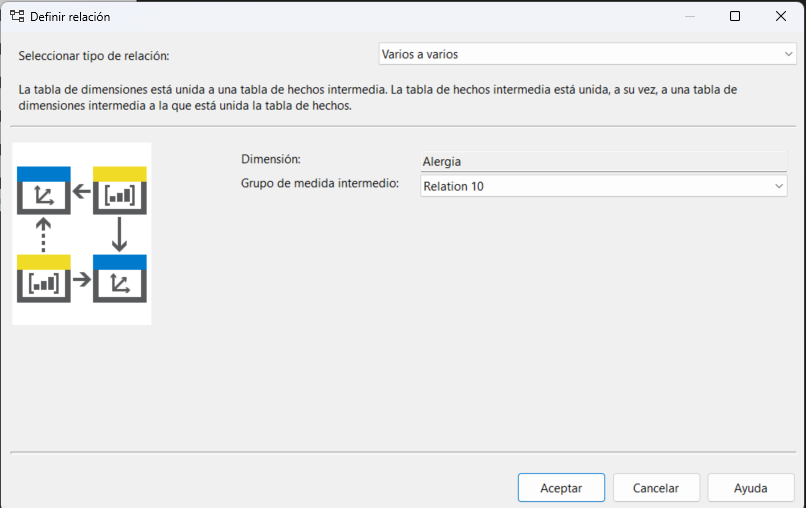
\includegraphics[width=.7\textwidth]{images/relation10.png}
		\caption{Configuración de relaciones de tipo Varios a Varios para Alergia.}
		\label{fig:relation10}
	\end{center}
\end{figure}

\begin{figure}[H]
	\begin{center} 
		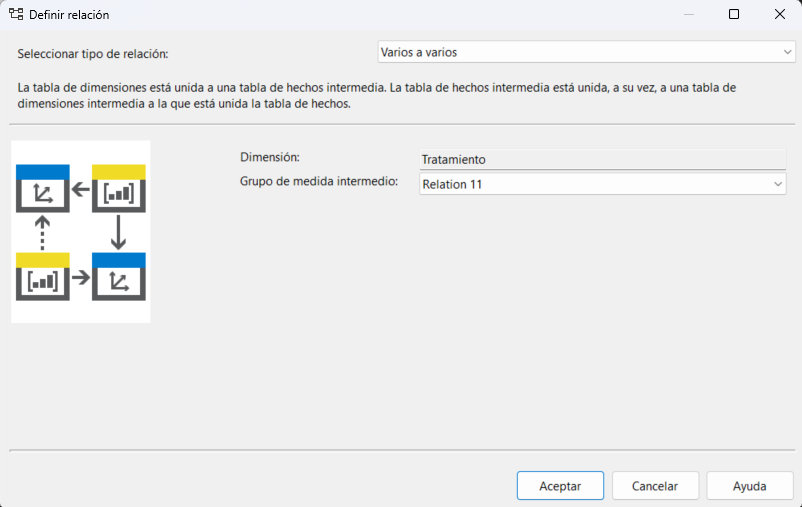
\includegraphics[width=.7\textwidth]{images/relation11.png}
		\caption{Configuración de relaciones de tipo Varios a Varios para Tratamiento.}
		\label{fig:relation11}
	\end{center}
\end{figure}

Al final de este proceso el esquema de uso de dimensiones quedará como en la figura \ref{fig:uso_dim}, donde las dimensiones alergia y tratamiento se relacionan con el gasto de medicamento de tipo varios a varios, pero para lograr esto las tablas intermedias(grupos de medidas intermedios) se tienen que relacionar con su dimension y el gasto.

\begin{figure}[H]
	\begin{center} 
		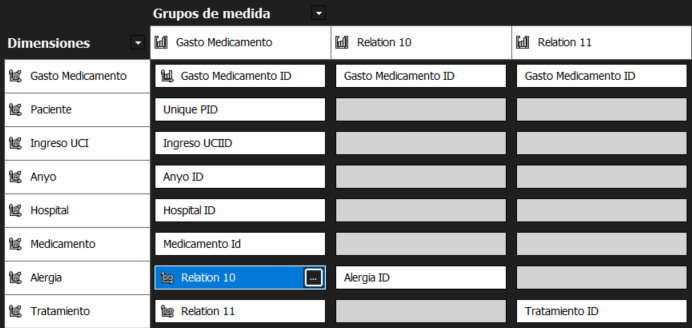
\includegraphics[width=.7\textwidth]{images/usoDimensiones.png} 
		\caption{Relaciones de dimensiones y grupos de medida del cubo.}
		\label{fig:uso_dim}
	\end{center}
\end{figure}
\subsection{Cálculo de Medidas}
La medida \textbf{Tasa de Infusión}, se deben calcular utilizando la media, el resto de medidas (cantidad, recuento de gasto y volumen de fluido) son aditivas.

\subsection{Jerarquías y Atributos}
Para cada tabla, organizamos las jerarquías con los IDs correspondientes, configuramos los \textbf{nameColumn} con identificadores claros y añadimos atributos adicionales que no se incluyan en las jerarquías.



\begin{itemize}
	\item \textbf{Paciente:} Configuramos la jerarquía con el ID de paciente, renombrado como \textit{Paciente}, y añadimos atributos como género y etnia. La figura \ref{fig:paciente_dim} muestra esta configuración.
	\item \textbf{Ingreso:} Configuramos la jerarquía con los IDs de ingreso en UCI y hospital, y añadimos atributos como fuente de admisión, estado de alta, tipo de unidad, altura y peso de admisión, como se muestra en la figura \ref{fig:ingreso_dim}.
	\item \textbf{Año:} Configuramos el atributo \textbf{nameColumn} para el nombre del año, como se muestra en la figura \ref{fig:anyo_dim}.
	\item \textbf{Hospital:} Se configura la jerarquía con el ID de región y el ID de hospital, renombrando estos como \textit{Región} y \textit{Hospital}, respectivamente. La región también tendrá su nombre referenciado. Los atributos de esta jerarquía incluirán el número de camas y el nombre de la región. La configuración se muestra en la figura \ref{fig:hospital_dim}.
	\item \textbf{Medicamento:} Esta dimensión será simple, ya que solo tendrá el ID y el nombre del medicamento, el cual se incluirá en el atributo \textbf{nameColumn}. La figura \ref{fig:medicamento_dim} muestra esta configuración.
	\item \textbf{Alergia:} La jerarquía se basará en el ID de alergia, renombrado como \textit{Alergia}, y el atributo \textbf{nameColumn} se usará para el nombre de la alergia. Además, se añadirán los atributos tipo de alergia y nombre de medicamento, en caso de que la alergia esté asociada a un medicamento. La configuración se muestra en la figura \ref{fig:alergia_dim}.
	\item \textbf{Tratamiento:} Se crea una jerarquía con el ID de tratamiento y la descripción del tratamiento, que se incluirá en el atributo \textbf{nameColumn} del ID. La figura \ref{fig:tratamiento_dim} muestra esta configuración.
\end{itemize}

\begin{figure}[H]
	\begin{center}
		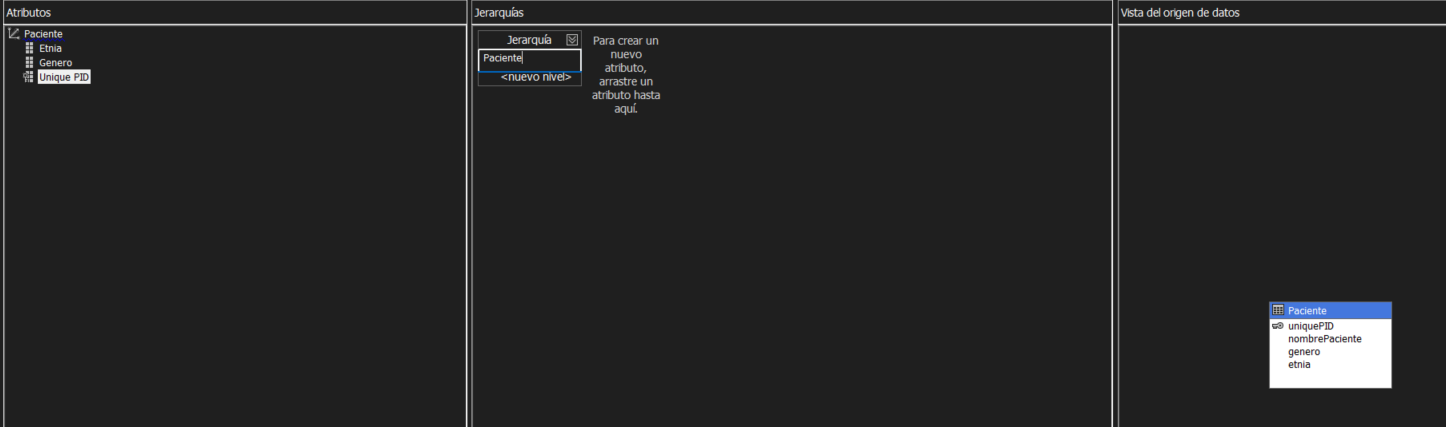
\includegraphics[width=0.8\textwidth]{images/paciente_dim.png}
		\caption{Jerarquías y atributos configurados para la tabla Paciente.}
		\label{fig:paciente_dim}
	\end{center}
\end{figure}

\begin{figure}[H]
	\begin{center}
		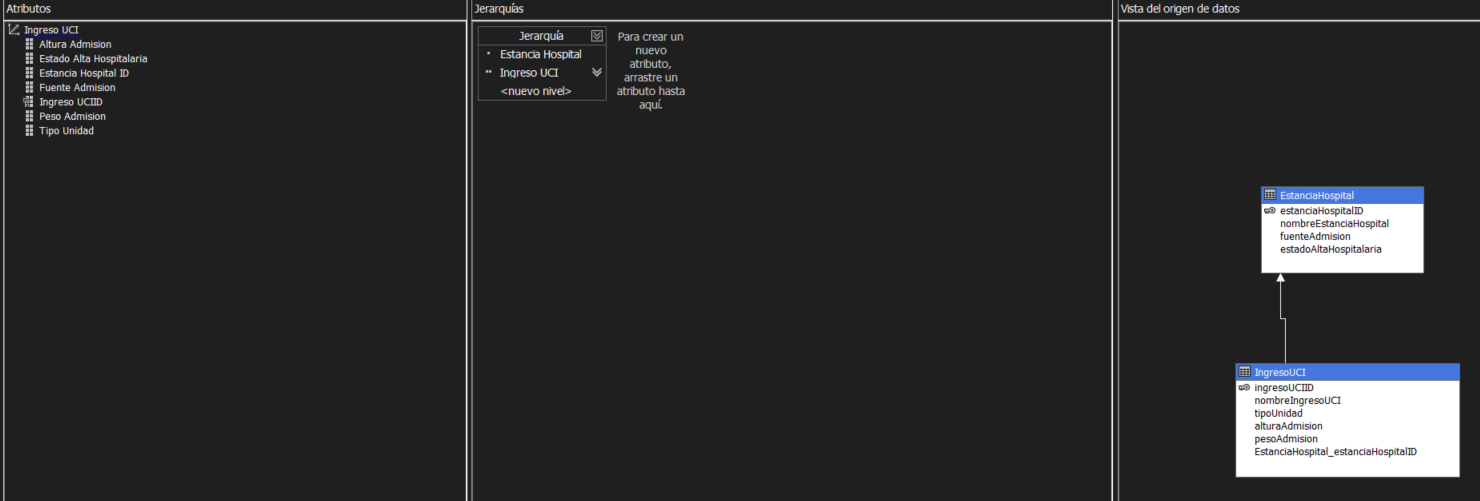
\includegraphics[width=0.8\textwidth]{images/ingreso_dim.png}
		\caption{Jerarquías configuradas para la tabla Ingreso.}
		\label{fig:ingreso_dim}
	\end{center}
\end{figure}

\begin{figure}[H]
	\begin{center}
		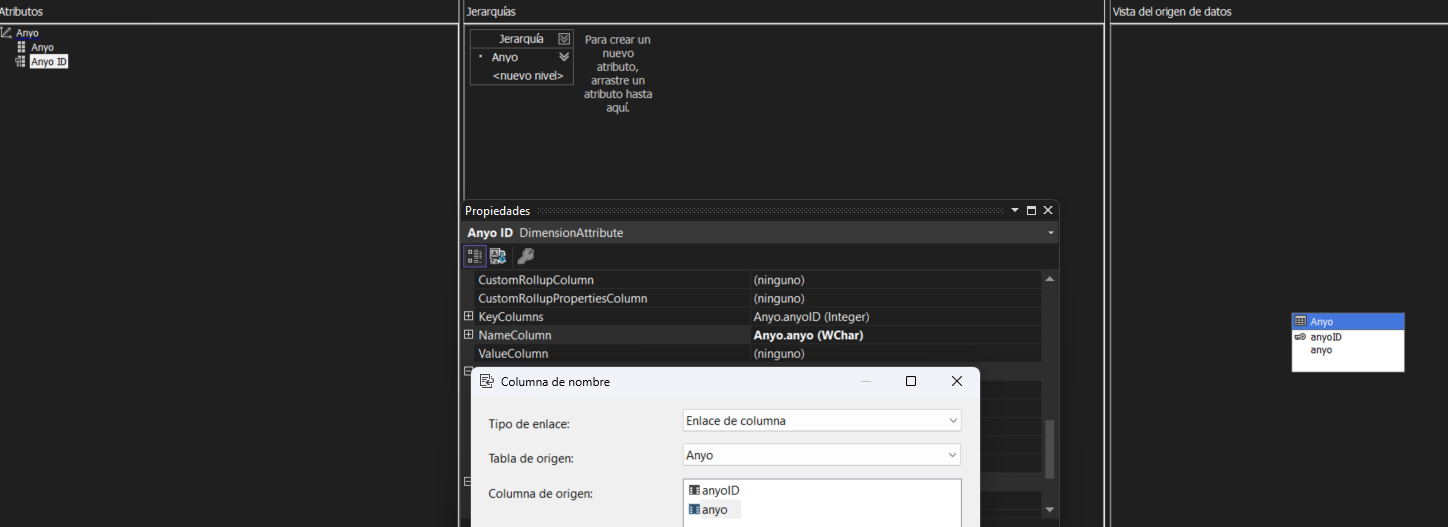
\includegraphics[width=0.8\textwidth]{images/anyo_dim.png}
		\caption{Configuración del atributo nameColumn para la tabla Año.}
		\label{fig:anyo_dim}
	\end{center}
\end{figure}

\begin{figure}[H]
	\begin{center}
		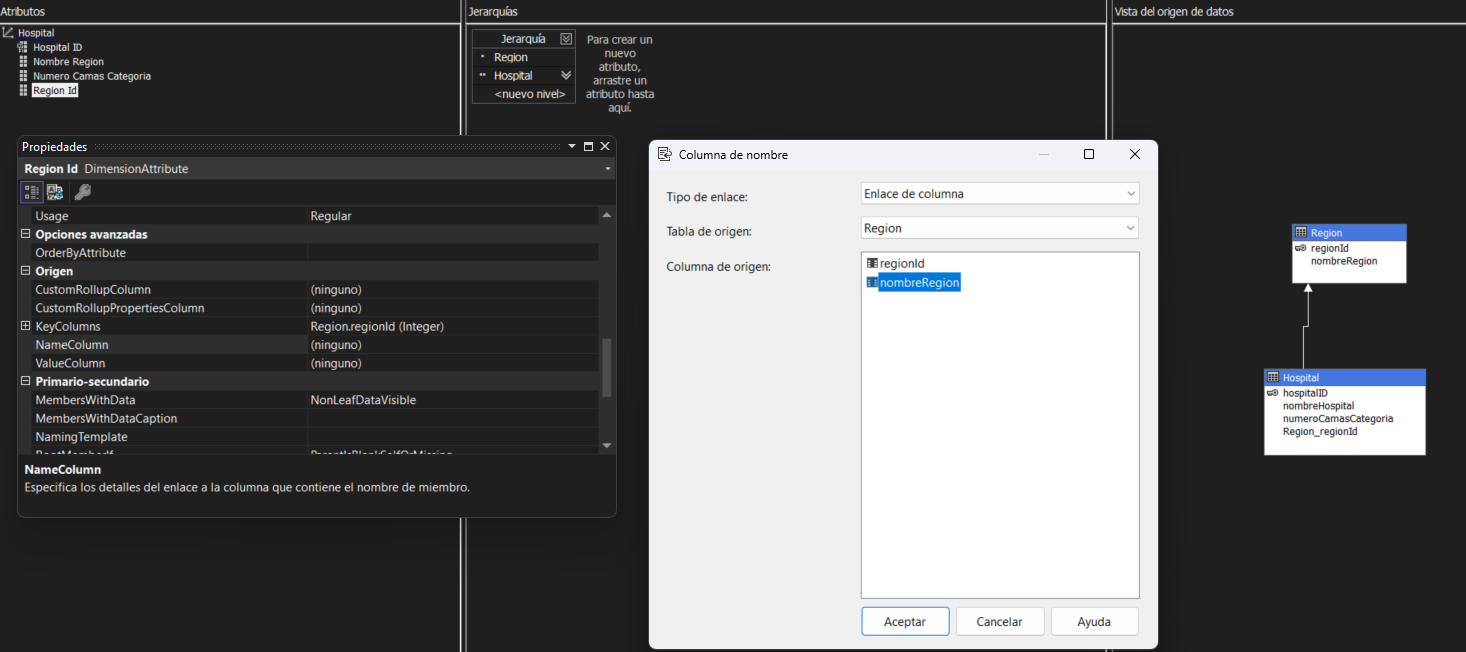
\includegraphics[width=0.8\textwidth]{images/hospital_dim.png}
		\caption{Jerarquías y atributos configurados para la tabla Hospital.}
		\label{fig:hospital_dim}
	\end{center}
\end{figure}

\begin{figure}[H]
	\begin{center}
		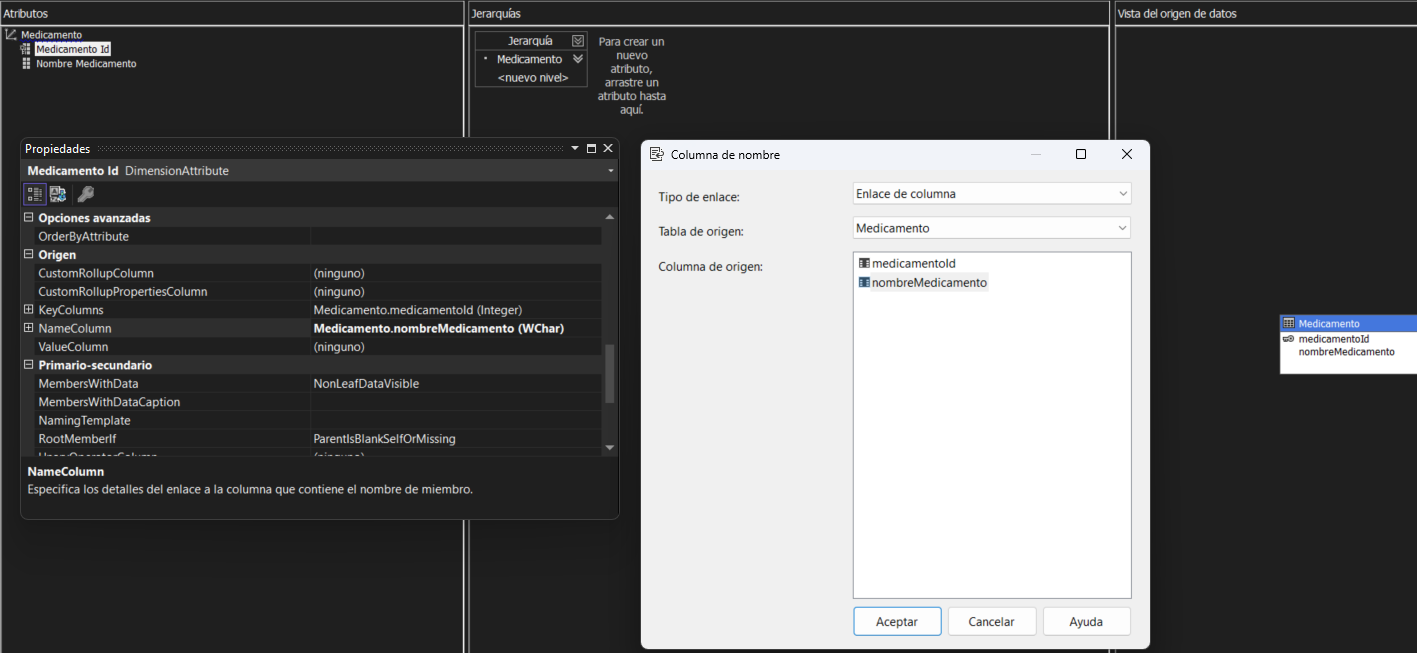
\includegraphics[width=0.8\textwidth]{images/medicamento_dim.png}
		\caption{Configuración de la tabla Medicamento con el ID y el nombre del medicamento.}
		\label{fig:medicamento_dim}
	\end{center}
\end{figure}

\begin{figure}[H]
	\begin{center}
		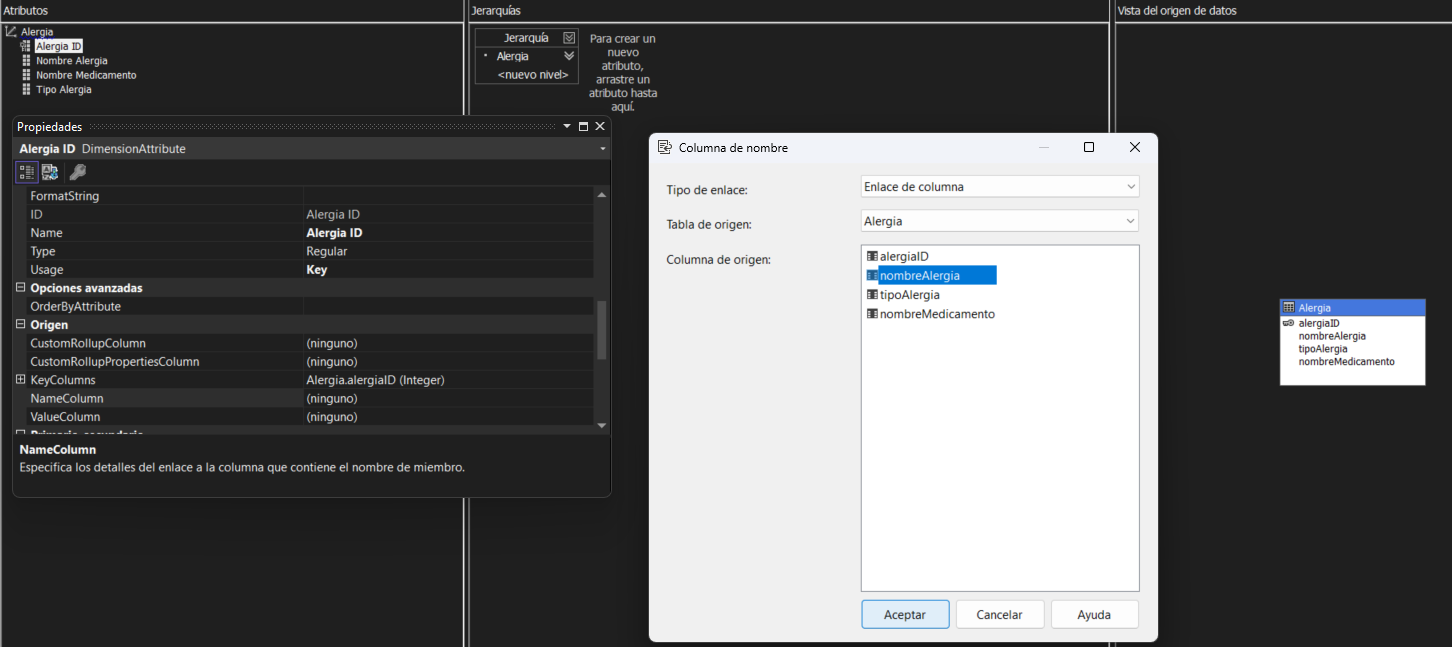
\includegraphics[width=0.8\textwidth]{images/alergia_dim.png}
		\caption{Jerarquías y atributos configurados para la tabla Alergia.}
		\label{fig:alergia_dim}
	\end{center}
\end{figure}

\begin{figure}[H]
	\begin{center}
		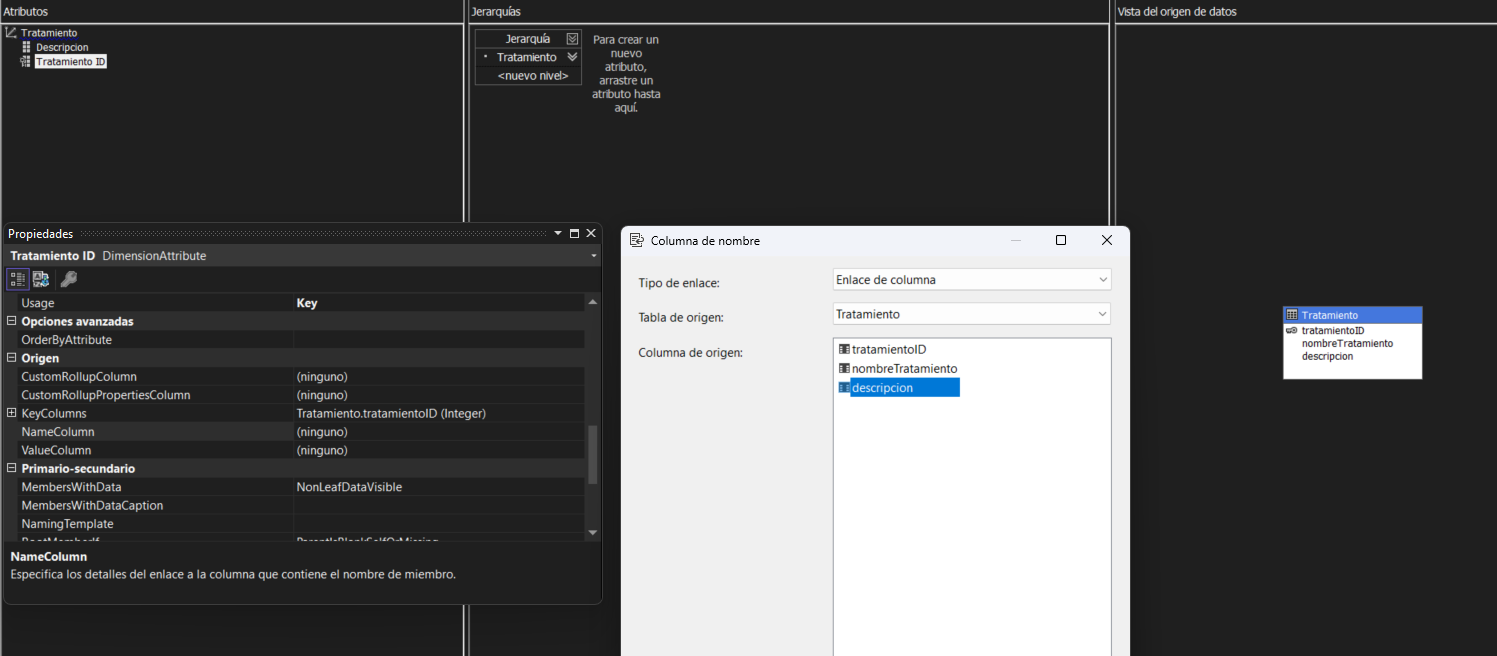
\includegraphics[width=0.8\textwidth]{images/tratamiento_dim.png}
		\caption{Jerarquías configuradas para la tabla Tratamiento.}
		\label{fig:tratamiento_dim}
	\end{center}
\end{figure}










\subsection{Procesamiento del Cubo}
Para procesar el cubo, haz clic derecho sobre él y selecciona la opción \textbf{Procesar}. En la figura \ref{fig:procesado_completo} se muestra el procesamiento del cubo.

\begin{figure}[H]
	\begin{center}
		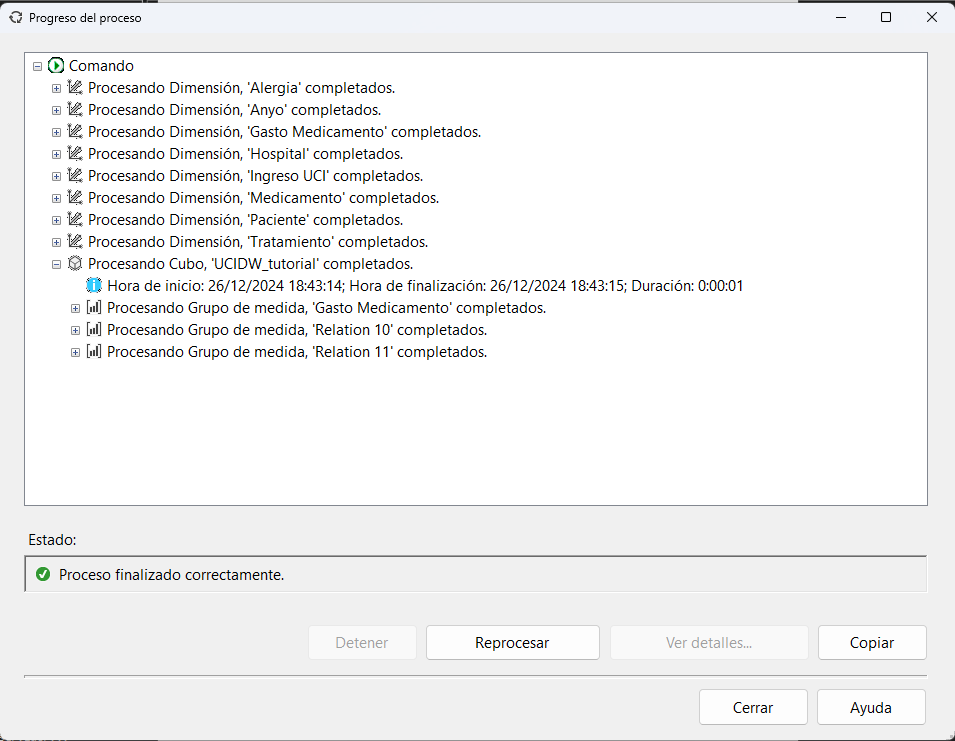
\includegraphics[width=0.8\textwidth]{images/procesado_completo.png}
		\caption{Procesamiento inicial del cubo multidimensional.}
		\label{fig:procesado_completo}
	\end{center}
\end{figure}

Para depurar errores, se recomieneda el procesamiento de manera secuencial con transacciones independientes.

\subsection{Conexión al Cubo Procesado}
Para acceder al cubo procesado, abre SQL Server, crea una conexión a Analysis Services en \textbf{localhost}, y navega hasta \textbf{Databases} para visualizar el cubo y realizar consultas MDX, como se muestra en la figura \ref{fig:conexion_cubo}.

\begin{figure}[H]
	\begin{center}
		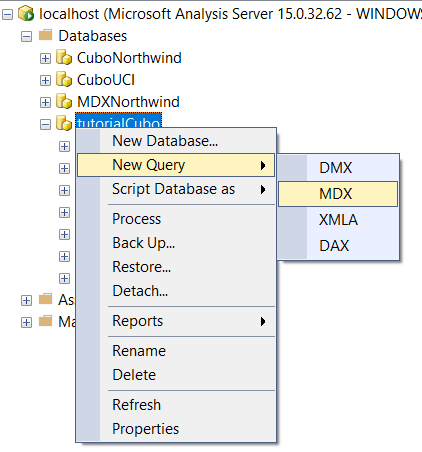
\includegraphics[width=0.5\textwidth]{images/conexion_cubo.png}
		\caption{Visualización del cubo en SQL Server tras la conexión a Analysis Services.}
		\label{fig:conexion_cubo}
	\end{center}
\end{figure}

\subsection{Verificación de Jerarquías}
Por último, verificamos las jerarquías creadas y navegamos por ellas para asegurarnos de que todo esté correcto, como se muestra en la figura \ref{fig:jerarquia}. 

\begin{figure}[H]
	\begin{center}
		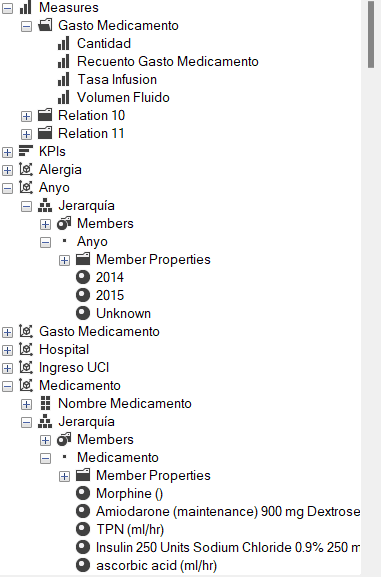
\includegraphics[width=0.5\textwidth]{images/navegacion.png}
		\caption{Verificación de jerarquías en el cubo multidimensional.}
		\label{fig:jerarquia}
	\end{center}
\end{figure}





	
	
	
	
	
	
	
	
	
	
	\section{Consultas MDX}
	A continuación, se muestran las consultas creadas para el cubo de Gasto de medicamentos en la UCI.

\subsection{Consulta 1}

\textbf{Ranking de Hospitales según Volumen de Fluido}
\\

Esta consulta en MDX genera un ranking de hospitales basado en el volumen de fluido, utilizando la base de datos multidimensional \texttt{[UCIDW]}. Primero, define una métrica calculada, \texttt{[Rank Volumen Fluido]}, que asigna un rango a cada hospital según el volumen de fluido (medida \texttt{[Measures].[Volumen Fluido]}) en orden descendente (\texttt{BDESC}). Luego, en la selección (\texttt{SELECT}), construye dos ejes: en las filas (\texttt{ON ROWS}), se muestran los hospitales que tienen un valor no vacío de volumen de fluido, ordenados ascendentemente por el ranking recién calculado (\texttt{BASC}). En las columnas (\texttt{ON COLUMNS}), se incluyen las medidas \texttt{[Volumen Fluido]} y \texttt{[Rank Volumen Fluido]}. 
\\
	
\begin{lstlisting}[style=ddlstyle, label=lst:consulta1,caption=Consulta 1: Ranking de Hospitales según Volumen de Fluido]


WITH 
	MEMBER [Measures].[Rank Hospitales] AS 
	RANK([Hospital].[Hospital].CURRENTMEMBER, 
	ORDER([Hospital].[Hospital].[Hospital].MEMBERS, 
	[Measures].[Volumen Fluido], BDESC))

SELECT 
	NON EMPTY 
		ORDER(
			FILTER(
				[Hospital].[Hospital].[Hospital].MEMBERS,
				NOT ISEMPTY([Measures].[Volumen Fluido])
			),
			[Measures].[Rank Hospitales],
			BASC
		) ON ROWS, 
	{[Measures].[Volumen Fluido], [Measures].[Rank Hospitales]} ON COLUMNS
FROM 
	[UCIDW]
\end{lstlisting}

\begin{figure}[H]
	\centering
	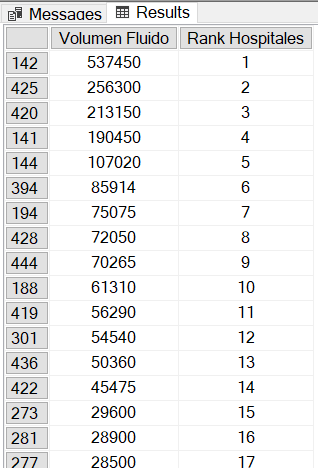
\includegraphics[width=0.35\linewidth]{images/consulta1.png}
	\caption{Resultados de la consulta 1: Ranking de Hospitales según Volumen de Fluido}
	\label{fig:consulta1}
\end{figure}

Como se muestra en la Figura \ref{fig:consulta1}, los resultados de la consulta presentan dos columnas principales: la primera indica el volumen de fluido correspondiente a cada hospital, mientras que la segunda muestra su posición en el ranking. Este ranking ordena los hospitales de manera descendente, desde el que registra el mayor gasto de fluido hasta el que registra el menor.


\subsection{Consulta 2}

\textbf{Tres medicamentos más gastados por cada unidad de UCI}
\\

Esta consulta en MDX identifica los tres medicamentos más utilizados en cada tipo de unidad de UCI. Primero, se define la métrica calculada \texttt{[Rank Medicamento]}, que asigna un ranking a cada medicamento dentro de su categoría según la cantidad utilizada (\texttt{[Measures].[Cantidad]}) en orden descendente (\texttt{BDESC}). En la selección (\texttt{SELECT}), se configuran dos ejes: en las columnas (\texttt{ON COLUMNS}), se incluye la medida \texttt{[Cantidad]}; y en las filas (\texttt{ON ROWS}), se genera una lista utilizando \texttt{TOPCOUNT} para seleccionar los tres medicamentos con mayor cantidad en cada tipo de unidad de UCI. Para lograr esto, se emplea \texttt{NONEMPTYCROSSJOIN} para cruzar los miembros actuales de las unidades de UCI con los medicamentos disponibles, y \texttt{NONEMPTY} para excluir combinaciones sin datos. 

Además para los medicamentos, se utilizó \texttt{.children} en lugar de \texttt{.MEMBERS} para evitar que apareciera el conjunto completo (\texttt{ALL}) como primera posición del ranking. Sin embargo, si se dejó en en el tipo de UCI para observar cuales son los medicamentos más utilizados en general.
\\

\begin{lstlisting}[style=ddlstyle, label=lst:consulta2,caption=Consulta 2: Tres medicamentos más gastados por cada unidad de UCI]
	
WITH 
	MEMBER [Measures].[Rank Medicamento] AS 
	RANK(
		[Medicamento].[Nombre Medicamento].CURRENTMEMBER,
		ORDER(
				[Medicamento].[Nombre Medicamento].children,
				[Measures].[Cantidad], 
			BDESC
			)
		)
	SELECT 
		{[Measures].[Cantidad]} ON COLUMNS, 
		NONEMPTY(
			GENERATE(
				[Ingreso UCI].[Tipo Unidad].members,
				TOPCOUNT(
					NONEMPTYCROSSJOIN(
						{[Ingreso UCI].[Tipo Unidad].CURRENTMEMBER}, 
						[Medicamento].[Nombre Medicamento].children
					), 
					3, 
					[Measures].[Cantidad]
				)
			)
		) ON ROWS
	FROM 
		[UCIDW]
\end{lstlisting}

En la Figura \ref{fig:consulta2} se presenta el resultado esperado de la consulta. Este muestra dos columnas principales: la primera enumera los tipos de unidades de UCI, mientras que la segunda identifica los medicamentos más utilizados en cada tipo específico de unidad. Además, junto a cada medicamento, se muestra la cantidad correspondiente, lo que permite un análisis detallado de su consumo en cada tipo de UCI.


\begin{figure}[H]
	\centering
	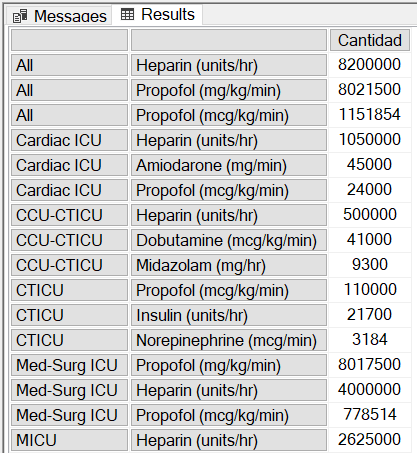
\includegraphics[width=0.4\linewidth]{images/consulta2.png}
	\caption{Resultados de la consulta 2: Tres medicamentos más gastados por cada unidad de UCI}
	\label{fig:consulta2}
\end{figure}


\subsection{Consulta 3}

\textbf{Cantidad de cada medicamento usado para hombres y para mujeres}
\\

Esta consulta en MDX calcula y muestra la cantidad de cada medicamento utilizado, desglosado por género (hombres y mujeres), utilizando nuevamente la base de datos multidimensional \texttt{[UCIDW]}. Define dos medidas calculadas: \texttt{[Cantidad Hombres]} y \texttt{[Cantidad Mujeres]}, que calculan la suma total de la cantidad de medicamentos consumidos por pacientes masculinos (\texttt{[Paciente].[Genero].[Male]}) y femeninos (\texttt{[Paciente].[Genero].[Female]}), respectivamente, utilizando la función \texttt{SUM}. En la cláusula \texttt{SELECT}, se configuran dos ejes: en las filas (\texttt{ON ROWS}), se listan los medicamentos disponibles (\texttt{[Medicamento].[Nombre Medicamento].MEMBERS}); y en las columnas (\texttt{ON COLUMNS}), se muestran las dos medidas calculadas (\texttt{[Cantidad Hombres]} y \texttt{[Cantidad Mujeres]}). 
\\

\begin{lstlisting}[style=ddlstyle, label=lst:consulta3,caption=Consulta 3: Cantidad de cada medicamento usado para hombres y para mujeres]
	
WITH 
	MEMBER [Measures].[Cantidad Hombres] AS
		SUM(
			{[Paciente].[Genero].[Male]}, 
			[Measures].[Cantidad]
		)
	MEMBER [Measures].[Cantidad Mujeres] AS
		SUM(
			{[Paciente].[Genero].[Female]}, 
			[Measures].[Cantidad]
		)
SELECT 
	NON EMPTY 
		{[Medicamento].[Nombre Medicamento].MEMBERS} ON ROWS,
		{[Measures].[Cantidad Hombres], [Measures].[Cantidad Mujeres]} ON COLUMNS
FROM 
	[UCIDW]
\end{lstlisting}

\begin{figure}[H]
	\centering
	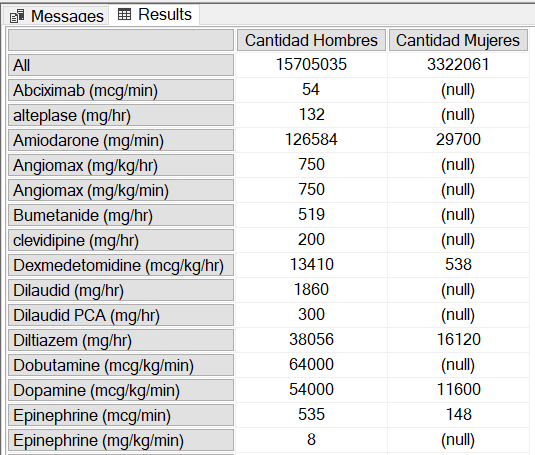
\includegraphics[width=0.5\linewidth]{images/consulta3.png}
	\caption{Resultados de la consulta 3: Cantidad de cada medicamento usado para hombres y para mujeres}
	\label{fig:consulta3}
\end{figure}

Como resultado, obtenemos dos columnas, una correspondiente a los hombres y otra a las mujeres (Figura \ref{fig:consulta3}), que muestran la cantidad de cada medicamento utilizado por cada género.



\subsection{Consulta 4}

\textbf{Pacientes con Mayor Uso de Medicamentos por Hospital (con mas de 500)}
\\

Esta consulta en MDX filtra los registros para mostrar únicamente aquellos en los que la cantidad de medicamento utilizada es superior a 500. En la cláusula \texttt{SELECT}, en las filas (\texttt{ON ROWS}), se combinan las jerarquías \texttt{[Hospital].[Hospital].[Hospital]} y los hijos de \texttt{[Paciente].[Unique PID].CHILDREN}, para evitar que se mostrara el total de pacientes como paciente con mayor uso de medicamentos. La función \texttt{FILTER} se utiliza para filtrar estas combinaciones, mostrando solo aquellas en las que la medida \texttt{[Measures].[Cantidad]} es mayor a 500. En las columnas (\texttt{ON COLUMNS}), se incluye la medida \texttt{[Measures].[Cantidad]}, que muestra la cantidad utilizada para cada combinación. 
\\


\begin{lstlisting}[style=ddlstyle, label=lst:consulta4,caption=Consulta 4: Pacientes con Mayor Uso de Medicamentos por Hospital (con mas de 500)]
	
SELECT 
	NON EMPTY 
		FILTER(
			[Hospital].[Hospital].[Hospital] * [Paciente].[Unique PID].CHILDREN,
			[Measures].[Cantidad] > 500
		) ON ROWS, 
		{[Measures].[Cantidad]} ON COLUMNS
FROM 
	[UCIDW]
\end{lstlisting}

\begin{figure}[H]
	\centering
	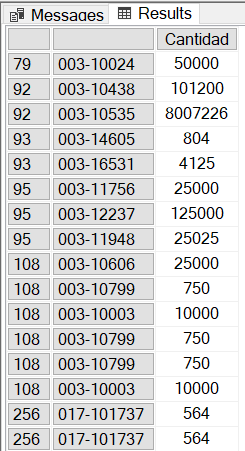
\includegraphics[width=0.3\linewidth]{images/consulta4.png}
	\caption{Resultados de la consulta 4: Pacientes con Mayor Uso de Medicamentos por Hospital (con mas de 500)}
	\label{fig:consulta4}
\end{figure}

El resultado es una tabla (Figura \ref{fig:consulta4}) que presenta solo aquellos hospitales y pacientes donde la cantidad de medicamento excede los 500. Se muestran dos columnas de filas, la primera representa los hospitales y la segunda los pacientes.

\subsection{Consulta 5}

\textbf{Volumen de fluido por tipo de UCI y tratamiento aplicado}
\\

Esta consulta en MDX muestra los tres tratamientos con los mayores volúmenes de fluido administrados para cada unidad de la UCI. En las columnas (\texttt{ON COLUMNS}), se seleccionan los hijos de \texttt{[Ingreso UCI].[Tipo Unidad].children}, que representan las distintas unidades de la UCI. En las filas (\texttt{ON ROWS}), se utiliza \texttt{TOPCOUNT} para identificar los tres tratamientos principales, basándose en los valores de la medida \texttt{[Measures].[Volumen Fluido]}. Para excluir combinaciones sin datos, se emplea la función \texttt{NONEMPTY}, que filtra únicamente las combinaciones relevantes. La consulta analiza el cubo \texttt{[UCIDW]} con la medida \texttt{[Measures].[Volumen Fluido]} como contexto en la cláusula \texttt{WHERE}, asegurando que todos los cálculos se centren en el volumen de fluido administrado.
\\ 

\begin{lstlisting}[style=ddlstyle, label=lst:consulta5,caption=Consulta 5: Volumen de fluido por tipo de UCI y tratamiento aplicado]
	
SELECT 
	[Ingreso UCI].[Tipo Unidad].children ON COLUMNS, 
	NONEMPTY(
		TOPCOUNT(
			[Tratamiento].[Descripcion].children, 
			3, 
			[Measures].[Volumen Fluido]
		)
	) ON ROWS
FROM 
	[UCIDW]
WHERE 
	[Measures].[Volumen Fluido]
\end{lstlisting}

\begin{figure}[H]
	\centering
	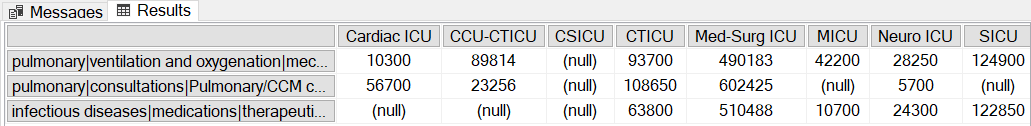
\includegraphics[width=0.9\linewidth]{images/consulta5.png}
	\caption{Resultados de la consulta 5: Volumen de fluido por tipo de UCI y tratamiento aplicado}
	\label{fig:consulta5}
\end{figure}

En la Figura \ref{fig:consulta5} se presentan los resultados de la quinta consulta, organizados en dos secciones principales. La primera sección muestra las diferentes unidades de la UCI representadas en las columnas, mientras que las filas presentan los tres tratamientos con los mayores volúmenes de fluido administrados, seleccionados para cada unidad. Para cada combinación de tratamiento y unidad, se indica el volumen de fluido correspondiente, destacando los tratamientos más relevantes en función de la medida \texttt{[Volumen Fluido]}. De este modo, los resultados permiten identificar los tratamientos más utilizados en cada unidad de la UCI según el volumen de infusión administrado.


\subsection{Consulta 6}

\textbf{Gasto medio de cantidad y volumen de fluido por numero de camas de hospitales}
\\

Esta consulta en MDX calcula el gasto medio de cantidad y volumen de fluido por categorías de número de camas en hospitales. Define dos medidas calculadas: \texttt{[Media Cantidad]} y \texttt{[Media Volumen Fluido]}, que utilizan la función \texttt{AVG} para calcular el promedio de las medidas \texttt{[Cantidad]} y \texttt{[Volumen Fluido]}. El uso de \texttt{EXISTING} es crucial, ya que asegura que los cálculos se limiten a la busqieda de los datos únicamente asociados a ese número de camas en concreto, evitando incluir datos del resto de categorías. En la cláusula \texttt{SELECT}, las medidas calculadas se muestran en las columnas (\texttt{ON COLUMNS}), mientras que las filas (\texttt{ON ROWS}) listan las categorías de número de camas mediante \texttt{[Hospital].[Numero Camas Categoria].CHILDREN}.
\\


\begin{lstlisting}[style=ddlstyle, label=lst:consulta6,caption=Consulta 6: Gasto medio de cantidad y volumen de fluido por numero de camas de hospitales]
	
WITH 
	MEMBER [Measures].[Media Cantidad] AS 
	AVG(
		EXISTING [Hospital].[Hospital].[Hospital].MEMBERS, 
		[Measures].[Cantidad]
	)
	MEMBER [Measures].[Media Volumen Fluido] AS 
	AVG(
		EXISTING [Hospital].[Hospital].[Hospital].MEMBERS, 
		[Measures].[Volumen Fluido]
	)
SELECT 
	{[Measures].[Media Cantidad], 
		[Measures].[Media Volumen
		Fluido]} ON COLUMNS, 
		[Hospital].[Numero Camas Categoria].CHILDREN ON ROWS
FROM 
	[UCIDW]
\end{lstlisting}

\begin{figure}[H]
	\centering
	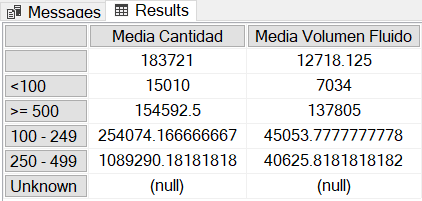
\includegraphics[width=0.5\linewidth]{images/consulta6.png}
	\caption{Resultados de la consulta 6: Gasto medio de cantidad y volumen de fluido por numero de camas de hospitales}
	\label{fig:consulta6}
\end{figure}

El resultado (Figura \ref{fig:consulta6}) muestra la media tanto de cantidad de gasto de medicamento como de volumen de fluido para cada cantidad de número de camas de los hospitales.

\subsection{Consulta 7}

\textbf{Gasto en medicamentos superior a 1000 por hospital, etnia, y año para pacientes masculinos en la UCI}
\\

En este caso, la consulta identifica los gastos en medicamentos superiores a 1000 para pacientes masculinos en la UCI, desglosados por hospital, etnia y año. Se define una medida calculada, \texttt{[Gasto Filtrado]}, que utiliza la función \texttt{IIF} para verificar si el gasto en medicamentos (\texttt{[Measures].[Cantidad]}) supera 1000; si es así, devuelve el valor de la medida, y en caso contrario, devuelve \texttt{NULL}. En la cláusula \texttt{SELECT}, en las filas (\texttt{ON ROWS}), se ordena la combinación de los años (\texttt{[Anyo].[Jerarquía].[Anyo]}), hospitales (\texttt{[Ingreso UCI].[Jerarquía].[Ingreso UCIID]}) y las etnias de los pacientes (\texttt{[Paciente].[Etnia].children}) en orden ascendente. En las columnas (\texttt{ON COLUMNS}), se incluye la medida \texttt{[Gasto Filtrado]}. Además, se aplica un filtro (\texttt{WHERE}) para limitar los resultados a pacientes masculinos (\texttt{[Paciente].[Genero].[Male]}). 

\begin{lstlisting}[style=ddlstyle, label=lst:consulta7,caption=Consulta 7: Gasto en medicamentos superior a 1000 por hospital etnia y año para pacientes masculinos en la UCI]
	
WITH 
	MEMBER [Measures].[Gasto Filtrado] AS 
	IIF([Measures].[Cantidad] > 1000, [Measures].[Cantidad], NULL)

SELECT 
	NON EMPTY 
		ORDER(
			{[Anyo].[Jerarquia].[Anyo].MEMBERS *
			[Ingreso UCI].[Jerarquia].[Ingreso UCIID].MEMBERS}*
			[Paciente].[Etnia].children, 
			[Anyo].[Anyo].CURRENTMEMBER, 
		ASC
		) ON ROWS, 
		{[Measures].[Gasto Filtrado]} ON COLUMNS
FROM 
	[UCIDW]
WHERE 
	([Paciente].[Genero].[Male])
\end{lstlisting}

El resultado es una tabla que detalla, para cada combinación de hospital, etnia y año, los gastos en medicamentos superiores a 1000 para pacientes masculinos en la UCI como se muestra a continuación.

\begin{figure}[H]
	\centering
	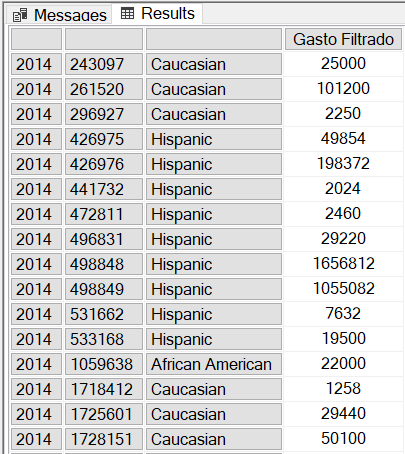
\includegraphics[width=0.4\linewidth]{images/consulta7.png}
	\caption{Resultados de la consulta 7: Gasto en medicamentos superior a 1000 por hospital, etnia, y año para pacientes masculinos en la UCI}
	\label{fig:consulta7}
\end{figure}


\subsection{Consulta 8}

\textbf{Volumen de fluido utilizado en el ingreso, clasificado por la altura y peso de los pacientes}
\\

La octava consulta calcula el volumen total de fluido utilizado para cada combinación de altura y peso de admisión en las unidades de UCI. Se define la medida calculada \texttt{[Volumen Fluido Utilizado]}, que utiliza la función \texttt{SUM} para sumar el volumen de fluido (\texttt{[Measures].[Volumen Fluido]}) a través de todos los tipos de unidad de UCI (\texttt{[Ingreso UCI].[Tipo Unidad].members}). En la cláusula \texttt{SELECT}, la medida \texttt{[Volumen Fluido Utilizado]} se coloca en las columnas (\texttt{ON COLUMNS}), mientras que las filas (\texttt{ON ROWS}) presentan las combinaciones de valores de altura y peso de admisión (\texttt{[Ingreso UCI].[Altura Admision].children} y \texttt{[Ingreso UCI].[Peso Admision].children}), generadas mediante \texttt{NONEMPTYCROSSJOIN} para excluir las combinaciones sin datos. 


\begin{lstlisting}[style=ddlstyle, label=lst:consulta8,caption=Consulta 8: Volumen de fluido utilizado en el ingreso clasificado por la altura y peso de los pacientes]
	
WITH 
	MEMBER [Measures].[Volumen Fluido Utilizado] AS 
	SUM(
		[Ingreso UCI].[Tipo Unidad].members, 
		[Measures].[Volumen Fluido]
	)
SELECT 
	{[Measures].[Volumen Fluido Utilizado]} ON COLUMNS,
	NONEMPTYCROSSJOIN(
		[Ingreso UCI].[Altura Admision].children, 
		[Ingreso UCI].[Peso Admision].children
	) ON ROWS
FROM 
	[UCIDW]
\end{lstlisting}


\begin{figure}[H]
	\centering
	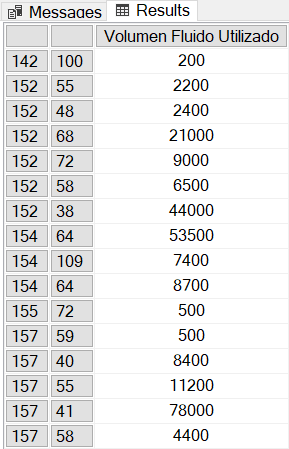
\includegraphics[width=0.3\linewidth]{images/consulta8.png}
	\caption{Resultados de la consulta 8: Volumen de fluido utilizado en el ingreso, clasificado por la altura y peso de los pacientes}
	\label{fig:consulta8}
\end{figure}

En la Figura \ref{fig:consulta8} podemos observar el resultado obtenido de la consulta con una columna que muestra el volumen de fluido clasificado en función de la altura (izquierda) y peso (derecha) de cada uno de los pacientes durante su ingreso.

\subsection{Consulta 9}

\textbf{Medicamentos que causan alergias y su gasto total}
\\

Esta consulta en MDX identifica los medicamentos que causan alergias y muestra la cantidad utilizada de estos. En la cláusula \texttt{SELECT}, en las columnas (\texttt{ON COLUMNS}), se incluye la medida \texttt{[Measures].[Cantidad]}, que representa el gasto total asociado a cada medicamento. En las filas (\texttt{ON ROWS}), se aplica la función \texttt{FILTER} para seleccionar únicamente aquellos medicamentos (\texttt{[Medicamento].[Nombre Medicamento].children}) que coinciden con los registrados en la dimensión de alergias (\texttt{[Alergia].[Nombre Medicamento].CURRENTMEMBER}). Esto asegura que solo se incluyan los medicamentos asociados con reacciones alérgicas.
\\

\begin{lstlisting}[style=ddlstyle, label=lst:consulta9,caption=Consulta 9: Medicamentos que causan alergias y su gasto total]
	
SELECT 
	{[Measures].[Cantidad]} ON COLUMNS, 
	FILTER(
		[Medicamento].[Nombre Medicamento].children, 
		[Alergia].[Nombre Medicamento].CURRENTMEMBER 
	) ON ROWS
FROM 
	[UCIDW]

\end{lstlisting}


\begin{figure}[H]
	\centering
	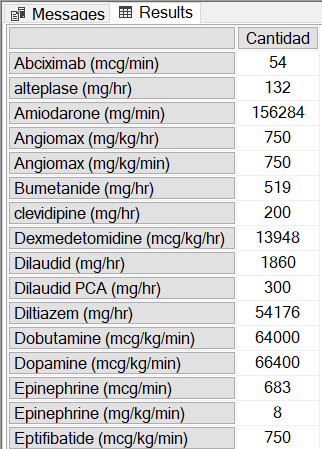
\includegraphics[width=0.3\linewidth]{images/consulta9.png}
	\caption{Resultados de la consulta 9: Medicamentos que causan alergias y su gasto total}
	\label{fig:consulta9}
\end{figure}

 El resultado observado en la Figura \ref{fig:consulta9} es una tabla que lista únicamente los medicamentos que causan alergias junto la cantidad utilizada de los mismos.
 
\subsection{Consulta 10}
\textbf{Volumen de fluido de cada medicamento por región en 2014}
\\

La décima muestra el volumen de fluido utilizado para cada medicamento en cada región concretamente el año 2014. En la cláusula \texttt{SELECT}, en las columnas (\texttt{ON COLUMNS}), se incluye la medida \texttt{[Measures].[Volumen Fluido]}, que representa el volumen total de fluido. En las filas (\texttt{ON ROWS}), se genera una combinación de regiones (\texttt{[Hospital].[Region].MEMBERS}) y medicamentos (\texttt{[Medicamento].[Nombre Medicamento].MEMBERS}) mediante la función \texttt{NONEMPTYCROSSJOIN}, que asegura que solo se incluyan combinaciones con datos disponibles. La cláusula \texttt{WHERE} restringe los resultados al año 2014 (\texttt{[Anyo].[Jerarquía].[Anyo].[2014]}).


\begin{lstlisting}[style=ddlstyle, label=lst:consulta10,caption=Consulta 10: Volumen de fluido de cada medicamento por region en 2014]
	
SELECT 
	{[Measures].[Volumen Fluido]} ON COLUMNS, 
	NONEMPTYCROSSJOIN(
		[Hospital].[Region].MEMBERS, 
		[Medicamento].[Nombre Medicamento].MEMBERS
	) ON ROWS
FROM 
	[UCIDW]
WHERE 
	([Anyo].[Jerarquia].[Anyo].[2014])

	
\end{lstlisting}


\begin{figure}[H]
	\centering
	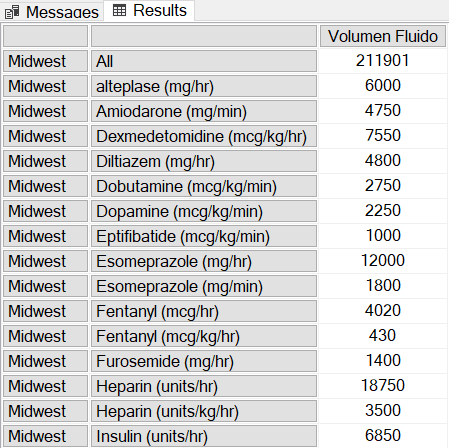
\includegraphics[width=0.4\linewidth]{images/consulta10.png}
	\caption{Resultados de la consulta 10: Volumen de fluido de cada medicamento por región en 2014}
	\label{fig:consulta10}
\end{figure}

Como resultado obtenemos la tabla de la figura \ref{fig:consulta10} donde se muestran los resultados de volumen de fluido clasificado por región de cada medicamento

\section{Tutorial ejecutar consultas}


	 Una vez tenemos el Cubo conectado a Analysis Services como se indica en la sección \textbf{\textit{Conexión al Cubo Procesado}}, seleccionamos el Cubo dentro de la carpeta Databases, pulsamos boton derecho y seleccionamos \textbf{New Query} en \textbf{MDX} como muestra la figura \ref{fig:conexion_cubo}.
	 
	 Aparecerá una pantalla donde pse podrán colocar una de las consultas de la lista como se muestra a continuación: 
	 
	 \begin{figure}[H]
	 	\centering
	 	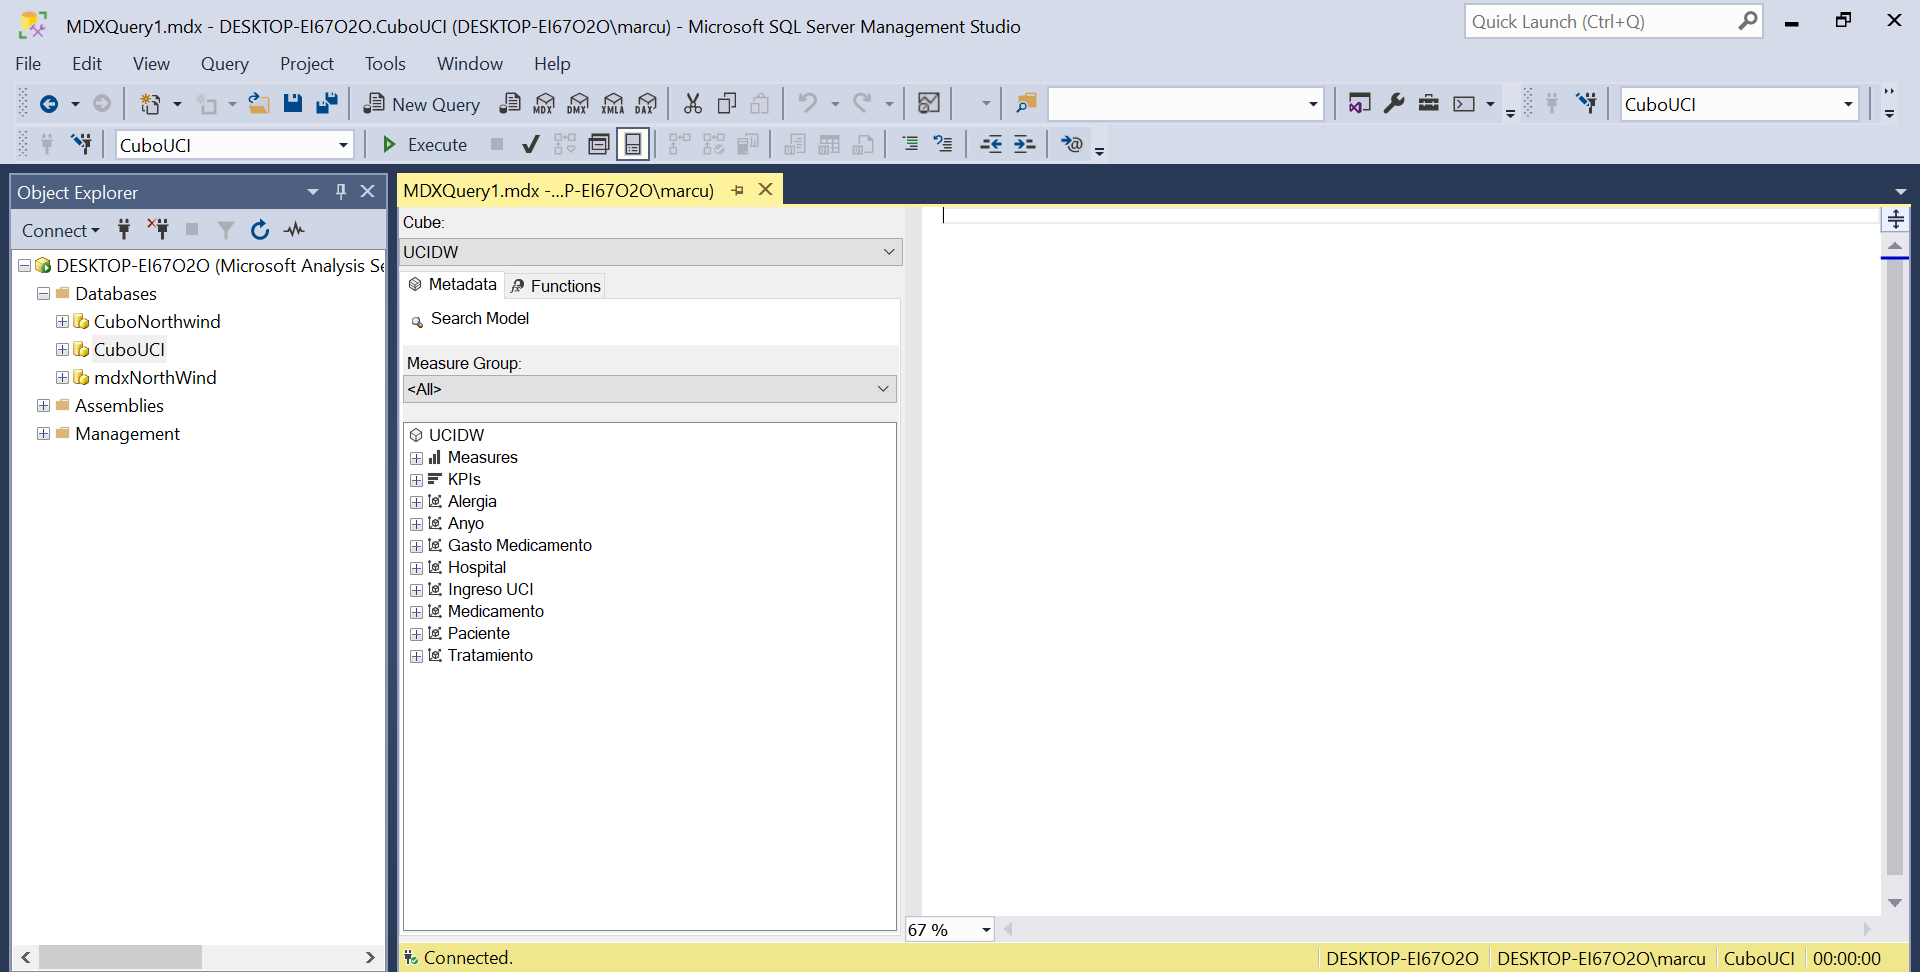
\includegraphics[width=1\linewidth]{images/pantallaconsulta.png}
	 	\caption{Pantalla de Analysis Services para la ejecución de una nueva consulta}
	 	\label{fig:pantallaconsulta}
	 \end{figure}
	 
	 Para ejecutar la consulta la se escribe la consulta en la pantalla y se pulsa el botón \textbf{Ejecutar} en verde.
	 
	 \begin{figure}[H]
	 	\centering
	 	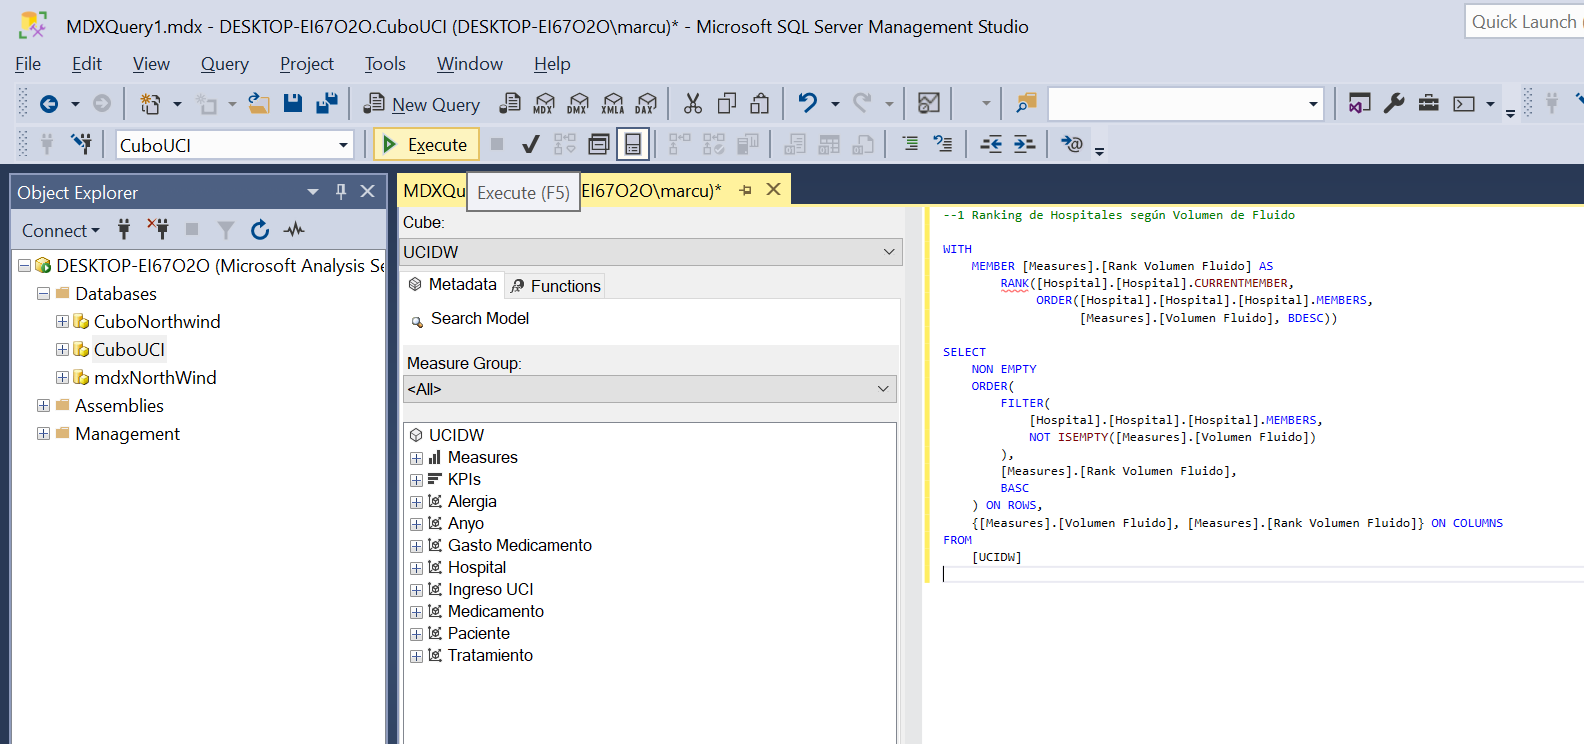
\includegraphics[width=1\linewidth]{images/ejecutar.png}
	 	\caption{Pantalla de Analysis Services para la ejecución la consulta escrito}
	 	\label{fig:ejecutar}
	 \end{figure}
	 
	  Tras pulsarlo este nos mostrará el resultado de la consulta en un cuadro de \textit{results} como el siguiente: 
	  
	  \begin{figure}[H]
	  	\centering
	  	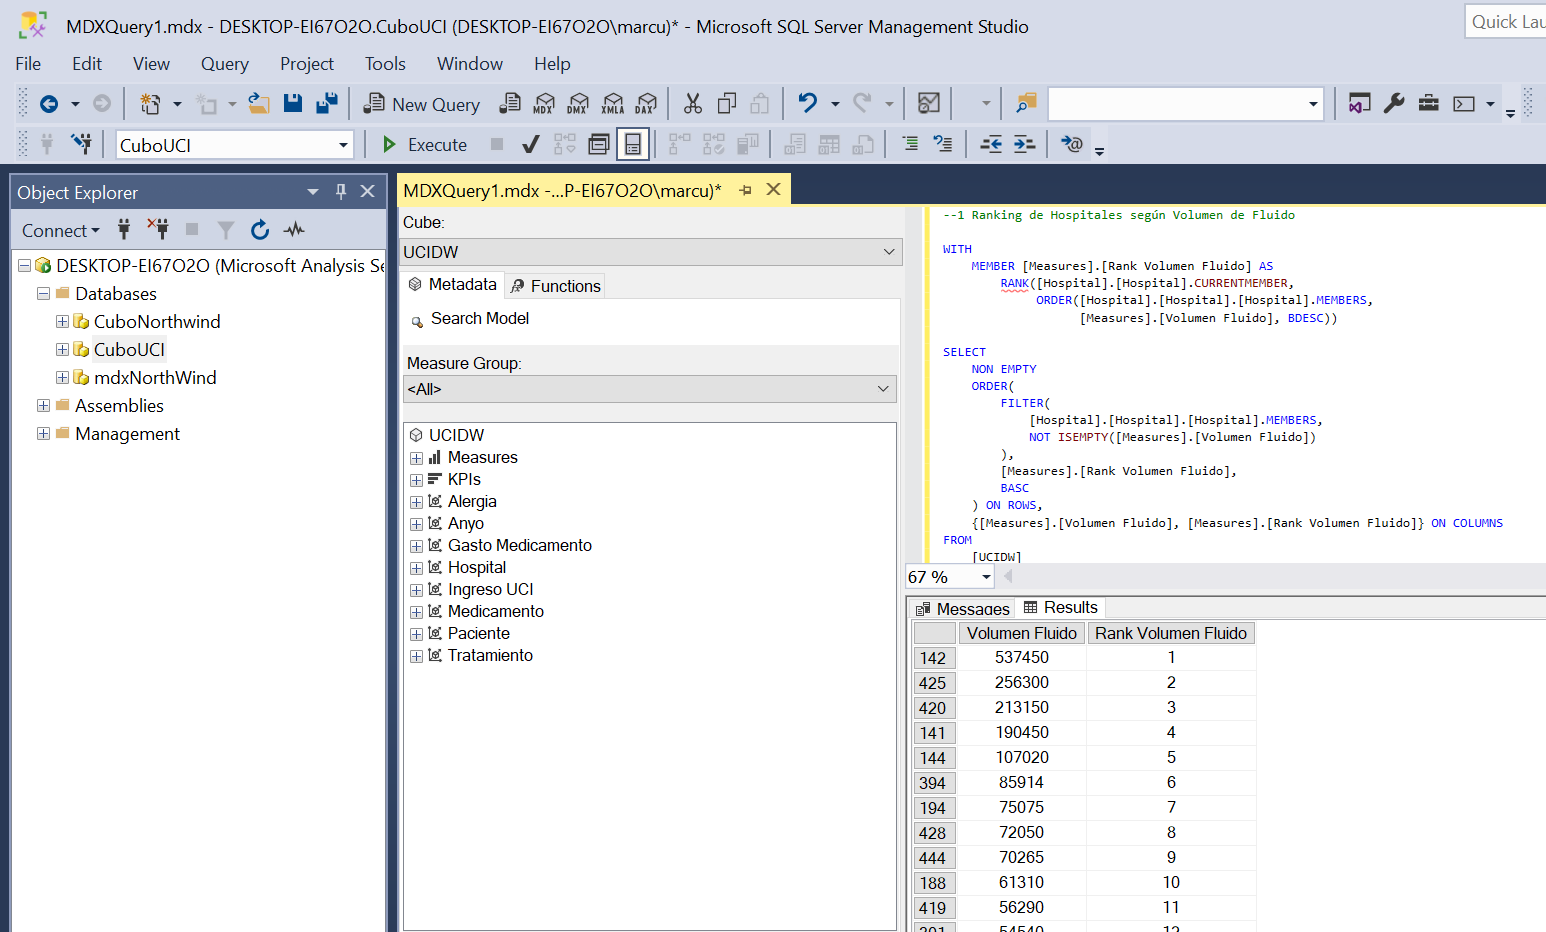
\includegraphics[width=1\linewidth]{images/resultado.png}
	  	\caption{Pantalla de Analysis Services para el resultado de la consulta}
	  	\label{fig:resultado}
	  \end{figure}
	 
	 \section{Dificultades Encontradas}
	 A lo largo de este proyecto, hemos enfrentado una serie de dificultades que, aunque han retrasado nuestro progreso, han resultado ser valiosas oportunidades de aprendizaje. 
	 
	 En la creación y procesamiento del cubo multidimensional de gasto de medicamento, uno de los principales desafíos ha sido la implementación de dimensiones con relaciones de varios a varios con el hecho, debido a la escasa documentación disponible sobre este tema. Esto nos obligó a investigar en profundidad y experimentar diferentes enfoques hasta encontrar una solución adecuada.
	 
	 Otra dificultad significativa surgió con el diseño inicial del cubo, que se demostró mejorable. Logramos formular consultas que aportan valor y sentido al almacén de gasto de medicamentos. 
	 
	 \section{Conclusión}
	 \label{sec:conclusion}
	 
	 La creación del cubo multidimensional de gasto de medicamento ha representado un paso clave en nuestro trabajo, construyendo sobre la base sólida establecida por el proceso ETL previo. Este proyecto no solo ha permitido estructurar los datos de manera más intuitiva y accesible, sino que también ha facilitado un análisis más profundo y específico del gasto farmacéutico.
	 
	 En conclusión, el cubo multidimensional desarrollado no solo ofrece una herramienta potente para el análisis del gasto de medicamentos, sino que también representa un avance importante en la construcción de infraestructuras de datos hospitalarios más robustas y orientadas al análisis avanzado.
	 
	\newpage
	\section{Acceso al Repositorio}
	
	Toda la información adicional, incluyendo el código fuente y la documentación completa de este proyecto, está disponible en el repositorio de GitHub \cite{silva2024github}.
	
	% Incluir la bibliografía
	\bibliographystyle{plain}  % Estilo de la bibliografía (por ejemplo, plain, alpha, ieee, etc.)
	\bibliography{bibli}  % Nombre del archivo .bib sin la extensión
	
\end{document}
